\documentclass[a4paper,12pt]{report}

\usepackage{alltt, fancyvrb, url}
\usepackage{graphicx}
\usepackage[utf8]{inputenc}
\usepackage{float}
\usepackage{hyperref}
\usepackage{markdown}

% Questo commentalo se vuoi scrivere in inglese.
\usepackage[italian]{babel}

\usepackage[italian]{cleveref}

\title{Relazione per\\"Bombardero: the Bomberman Remake"}

\author{Bello Figo Gu}
\date{\today}


\begin{document}

\maketitle

\begin{abstract}
Questo documento è una relazione di meta livello, ossia una relazione che spiega come scrivere la relazione.
%
Lo scopo di questo documento è quello di aiutare gli studenti a comprendere quali punti trattare nella loro relazione, ed in che modo farlo, evitando di perdere del tempo prezioso in prolisse discussioni di aspetti marginali tralasciando invece aspetti di maggior rilievo.
%
Per ciascuna delle sezioni del documento sarà fornita una descrizione di ciò che ci si aspetta venga prodotto dal team di sviluppo, assieme ad un elenco (per forza di cose non esaustivo) di elementi che \emph{non} dovrebbero essere inclusi.

Il modello della relazione segue il processo tradizionale di ingegneria del software fase per fase (in maniera semplificata).
%
La struttura della relazione non è indicativa ma \textit{obbligatoria}.
%
Gli studenti dovranno produrre un documento che abbia la medesima struttura, non saranno accettati progetti la cui relazione non risponda al requisito suddetto.
%
Lo studente attento dovrebbe sforzarsi di seguire le tappe suggerite in questa relazione anche per l'effettivo sviluppo del progetto: oltre ad una considerevole semplificazione del processo di redazione di questo documento, infatti, il gruppo beneficerà di un processo di sviluppo più solido e collaudato, di tipo top-down.

La meta-relazione verrà fornita corredata di un template \LaTeX{} per coloro che volessero cimentarsi nell'uso.
%
L'uso di \LaTeX{} è vantaggioso per chi ama l'approccio ``what you mean is what you get'', ossia voglia disaccoppiare il contenuto dall'effettivo rendering del documento, accollando al motore \LaTeX{} l'onere di produrre un documento gradevole con la struttura ed il contenuto forniti.
%
Chi non volesse installare l'ambiente di compilazione in locale può valutare l'utilizzo dell'applicazione web \href{https://www.overleaf.com/}{Overleaf}.
%
L'eventuale utilizzo di \LaTeX{} non è fra i requisiti,
non è parte del corso di Programmazione ad Oggetti, e non sarà ovviamente valutato.
%
I docenti accetteranno qualunque relazione in formato standard Portable Document Format (pdf) o Markdown (md), indipendentemente dal software con cui tale documento sarà redatto.

Per la realizzazione degli schemi UML, si raccomanda l'utilizzo di MermaidJS\footnote{\url{https://mermaid.live/}} o PlantUML \footnote{\url{https://plantuml.com/}}.
%
Gli schemi in questa relazione furono realizzati con StarUML.
%
Come per la prosa, non è importante quale strumento sia utilizzato, ma è vitale che gli schemi siano di buona qualità e ben leggibili.

\end{abstract}

\tableofcontents

\chapter{Analisi}
\section{Requisiti}
Il collettivo mira alla creazione di un videogioco ispirato alla nota saga videoludica “Bomberman”.
Il giocatore controlla un personaggio, in grado di muoversi liberamente nei confini della mappa e di piazzare delle bombe. L’obiettivo generale del gioco è quello di sconfiggere i nemici presenti sulla mappa piazzando strategicamente gli esplosivi, in grado di far saltare in aria eventuali ostacoli.

\subsection*{Requisiti funzionali}
\begin{itemize}
	\item L'applicazione dovrà fornire un ambiente di gioco virtuale rappresentato da una griglia bidimensionale. La griglia dovrà essere suddivisa in celle nelle quali i giocatori potranno muoversi solo orizzontalmente o verticalmente.
            \begin{itemize}La griglia verrà riempita da due tipologie di ostacoli:
                \item Muri indistruttibili: generati in maniera fissa a scacchiera
                \item Muri deboli: che verranno piazzati casualmente per riempire parzialmente i restanti spazi vuoti della griglia
            \end{itemize}
	\item Dopo un minuto e mezzo dall’inizio della partita i muri indistruttibili che formano il confine dell’arena inizieranno a collassare verso il centro, riducendo l’area calpestabile ed eliminando i giocatori che si trovano nelle loro prossimità al momento del crollo. I muri cominciano il loro crollo a partire dall’angolo in basso a sinistra, uno per volta, procedendo in senso orario.
	\item Si dovrà implementare un giocatore principale, controllabile da parte dell’utente mediante tastiera utilizzando i tasti W, A, S e D rispettivamente per il movimento verso l’alto, verso il sinistra, verso il basso e verso destra. Verrà utilizzato il tasto B per il piazzamento delle bombe.
	\item Dovranno essere presenti tre nemici, controllati dal computer, il cui scopo sarà quello di sconfiggere gli altri giocatori presenti nella mappa.
	\item Ogni entità presente potrà piazzare delle bombe nella propria posizione corrente, che esploderanno dopo qualche secondo (permettendo ai giocatori di allontanarsi)
        \item L’esplosione causerà delle fiamme, che espandendosi verticalmente e orizzontalmente per un certo numero di caselle, cambieranno la conformazione dell’arena e danneggeranno le entità vicine. Inoltre, se la fiamma di una bomba ne colpisce un’altra, allora anche quest'ultima dovrà esplodere innestando un effetto a catena.
        \item Normalmente, una volta piazzata una bomba in una cella non sarà possibile attraversarla fino a quando essa non esplode. 
        \item I giocatori possono attraversare celle in cui sono presenti anche altri player senza che essi presentino un ostacolo.
        \item Saranno presenti ostacoli nella griglia (muri deboli), che potranno essere distrutti dalle esplosioni delle bombe, permettendo al personaggio di passare attraverso lo spazio vuoto appena creato, diversamente dai muri indistruttibili che non potranno essere alterati.
        \item Dalle esplosioni degli ostacoli si possono generare degli oggetti speciali (power up oppure dei malus), che cambieranno le abilità delle singole entità. Per ottenerli basterà raccoglierli passandoci sopra.
        \item Il software deve includere una breve guida che insegni all'utente come giocare e come muoversi all'interno del gioco
\end{itemize}

\subsection*{Requisiti non funzionali}
\begin{itemize}
    \item L’applicazione dovrà essere ottimizzata al fine di permettere un’esperienza di gioco fluida 
\end{itemize}

\section{Analisi e modello del dominio}

L'arena di gioco detta \verb|Game Map| sarà composta da \verb|Cell|. 
Queste \verb|Cell| potranno essere di diverso tipo: 

\begin{itemize}
    \item Muri indistruttibili, chiamati nel dominio \verb|Unbreakable Wall|
    \item Muri distruttibili, chiamati nel dominio \verb|Breakable Wall|
    \item Potenziamenti, che possono essere raccolti dai \verb|Character|, chiamati nel dominio \verb|PowerUp|
    \item Bombe, chiamate nel dominio \verb|Bomb|
    \item Fiamme, generate dall'esposione delle bombe chiamate nel dominio \verb|Flame|
\end{itemize}

\begin{figure}[h]
\centering{}
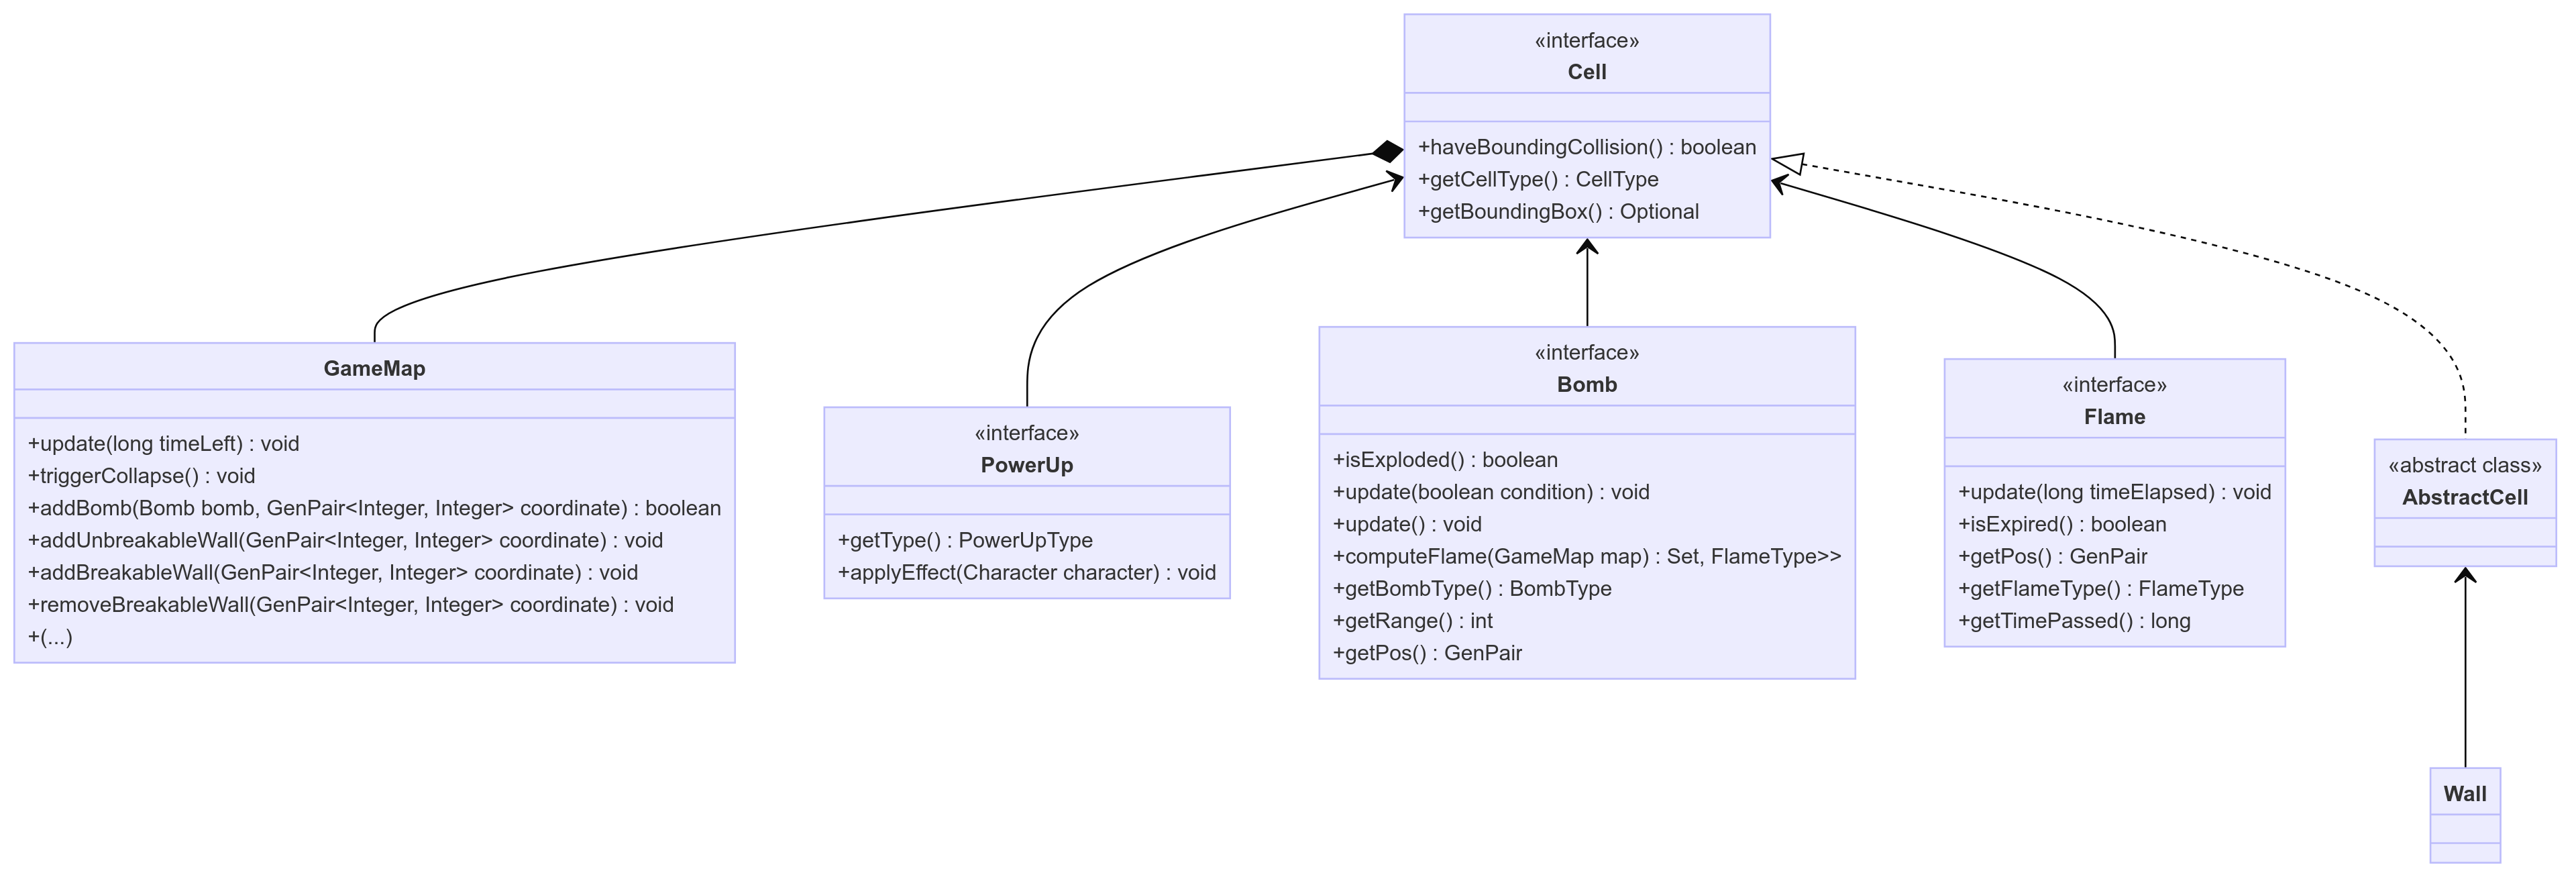
\includegraphics[width=\textwidth]{img/interface-cell.png}
\caption{Schema UML sulle relazioni tra le varie entità di tipo Cell}
\end{figure}

Il \verb|Character| si divide in \verb|Player| e \verb|Enemy|. Qualsiasi personaggio può piazzare delle bombe sulle celle libere della mappa che una volta esplose generano una serie di fiamme. Le fiamme interagiscono con i muri, con i potenziamenti e con le bombe modificando la struttura della mappa, distruggendo ciò che ci trova nella stessa Cell ed espandendosi attraverso le celle libere. Un muro, se distrutto, può lasciare un potenziamento al suo posto. 

Il tutto viene racchiuso nell'interfaccia \verb|GameManager|, di cui si parlerà in dettaglio nella prossima sezione, nella seguente maniera: 

\begin{figure}[h]
\centering{}
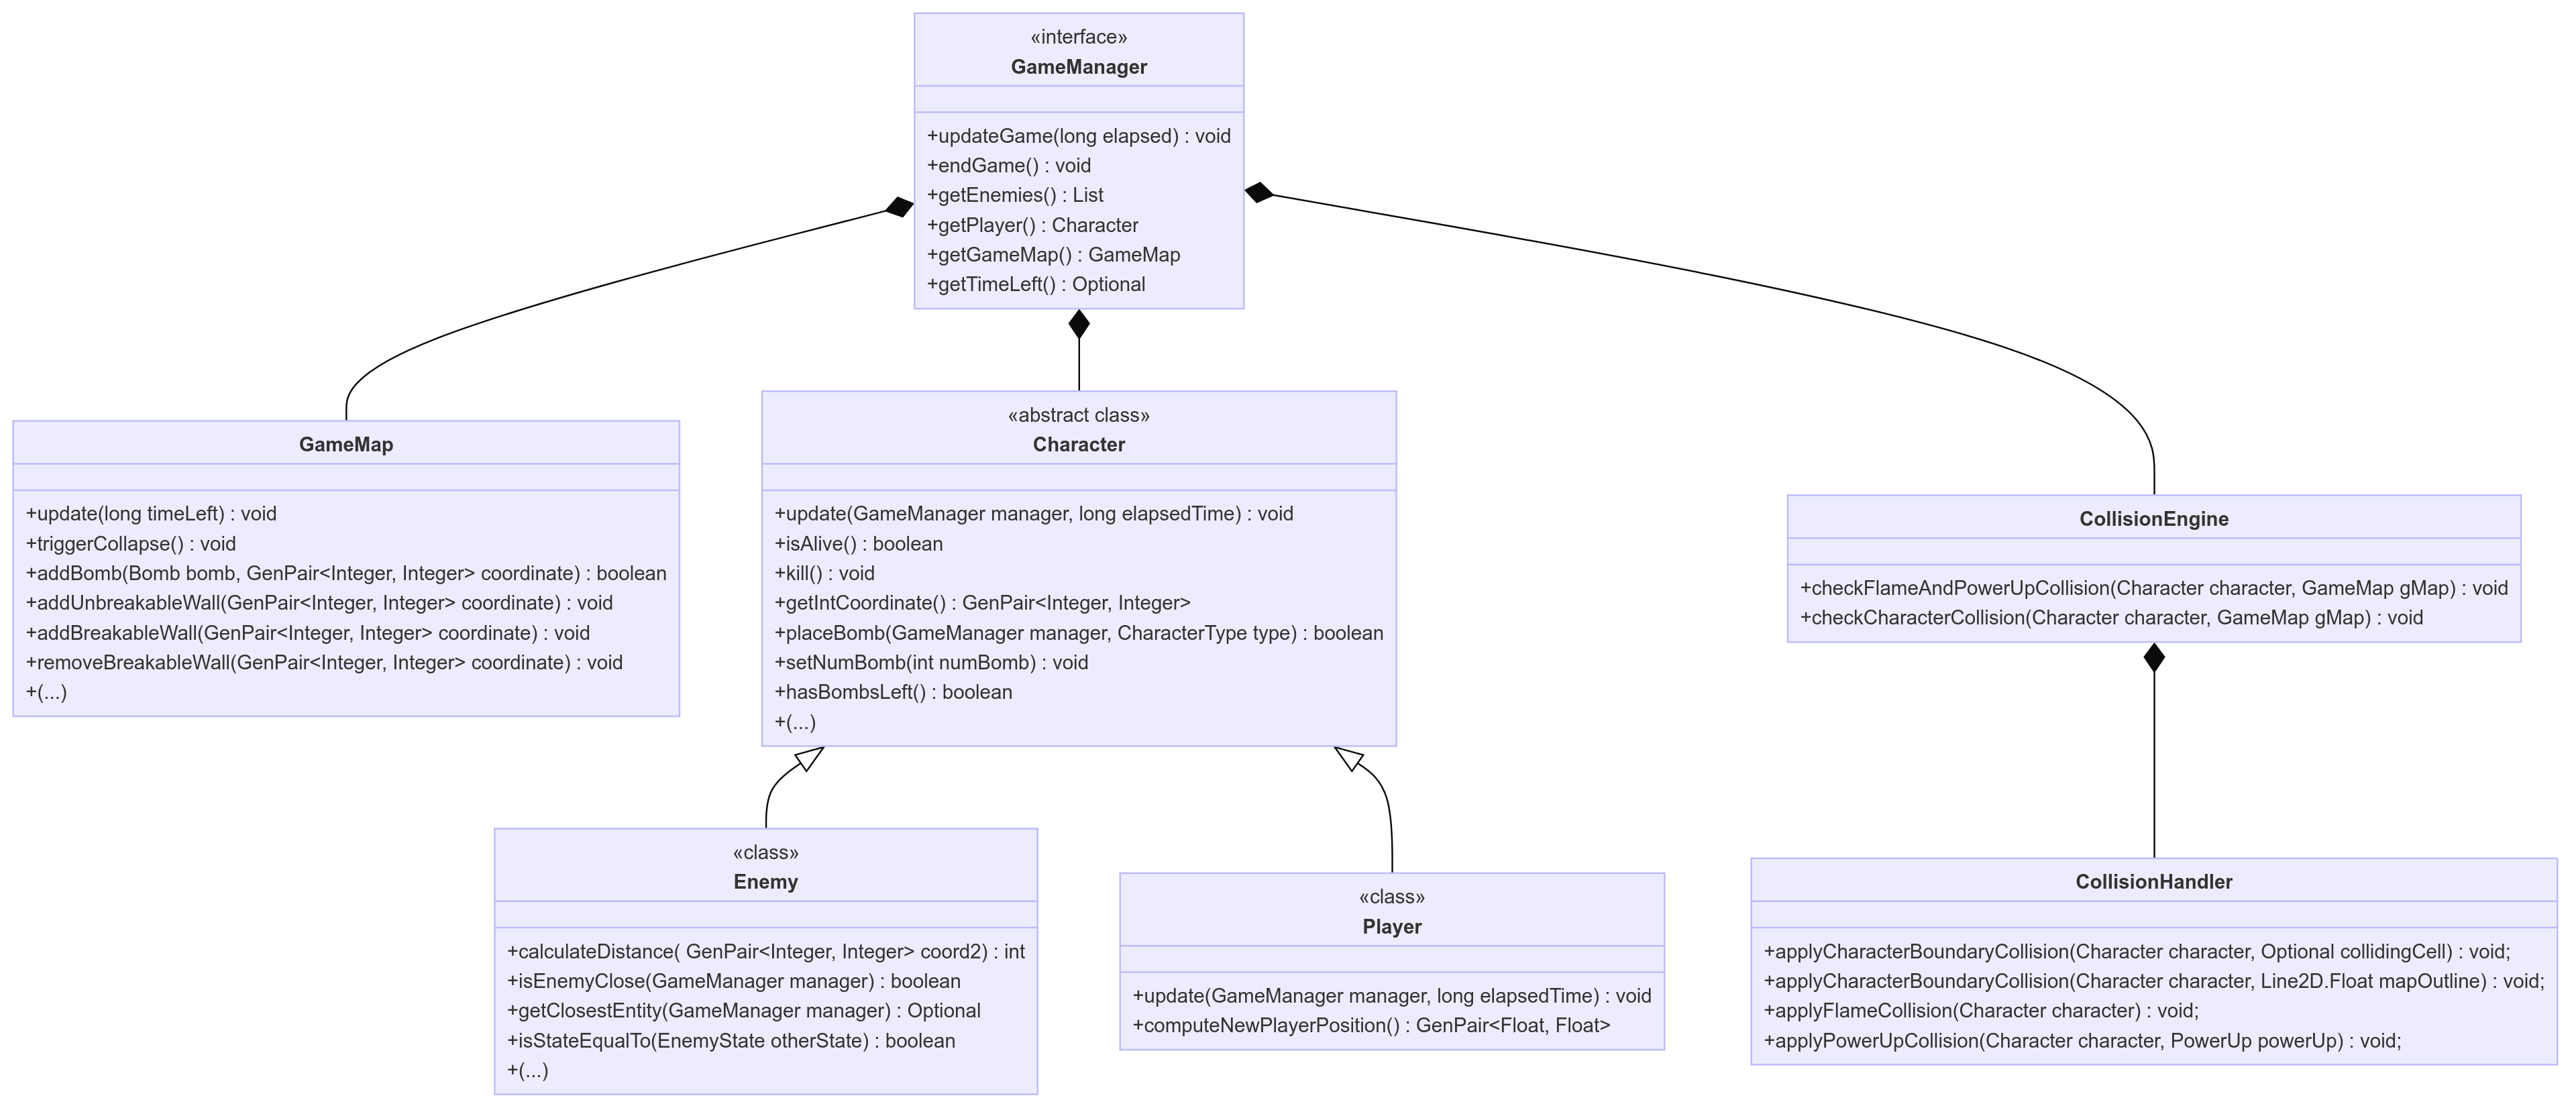
\includegraphics[width=\textwidth]{img/manager-riassunto.png}
\caption{Schema UML riassuntivo sulla composizione generale del model}
\end{figure}

\chapter{Design}

\section{Architettura}

In questo applicativo è stato utilizzato il pattern architetturale model-view-controller. Le interfacce che compongono in pattern sono \verb|Controller|, \verb|GraphicsEngine| e 
\verb|GameManager| mentre per quanto riguarda il game loop necessario ad aggiornare ciclicamente le componenti di gioco sia di model che di view è stata creata l'interfaccia \verb|Engine|.
\par
L'interfaccia \verb|GameManager| è il punto d'ingresso al model. Si occupa dell'aggiornamento degli aspetti dinamici delle componenti del dominio e della gestione delle dinamiche di gioco.
\par
\verb|Controller| è l'interfaccia rappresentante omonimo componente dell'architettura M.V.C. esso fa da tramite tra la view, rappresentata da \verb|GraphicsEngine|, \verb|GameManager| e l'interfaccia di gestione degli input dell'utente \verb|KeyListener| 

\begin{figure}[h]
\centering{}
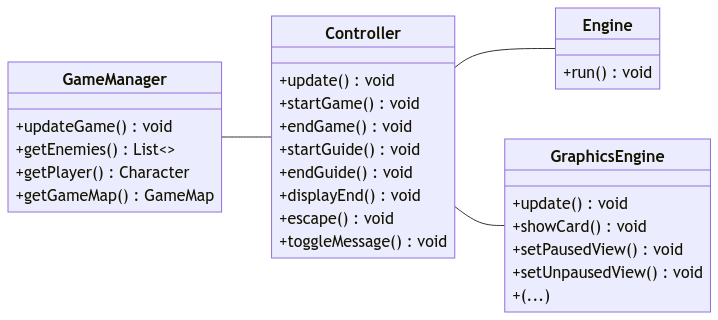
\includegraphics[width=\textwidth]{img/mvc.png}
\caption{Schema UML riassuntivo dell'architettura M.V.C. dell'applicativo}
\end{figure}

\par 
Per quanto riguarda la indipendenza degli elementi di questa architettura l'interfaccia grafica, il controller mette a disposizione i metodi necessari per poter comunicare all'interfaccia grafica quali sono gli elementi da mostrare. A sua volta l'interfaccia grafica mette a disposizione diversi metodi per permettere al controller di modificare la vista ed impostare visuali diverse.

\section{Design dettagliato}

\subsection{qualcosa di Federico Bagattoni}
\subsection{Luca Venturini}
\subsection*{1. Problema da Risolvere}

\par
Fare in modo che i personaggi all'interno dell'arena non possano oltrepassare i muri della mappa e aluni tipi di Cell utilizzando un movimento su un piano continuo.
%
\subsection*{1. Soluzione Proposta}

\begin{figure}[H]
\centering{}
\includegraphics[width=\textwidth]{report-src/img/RectangleBox.png}
\caption{Schema UML riassuntivo della classe RectangleBoundingBox}
\end{figure}

\par
Per risolvere questo problema è stato utilizzato il pattern \verb|Adapter| dove la classe RectangleBoundingBox si compone di un Rectangle2D per descrivere la parte solida di un Character o di una Cell, di fatto RectangleBoundingBox utilizza i metodi di un Rectangle2D per ricavare informazioni utili, come nel caso di una collisione la distanza che il Character deve percorrere per non collidere più rispetto ad un muro.
Con questa implementazione si lascia poco spazio a nuove BoundingBox magari di forme diverse, però abbiamo valutato che in questo caso sia appropriata dati gli elementi di gioco presenti nel dominio e l'utilizzo che ne viene fatta.


\begin{figure}[H]
\centering{}
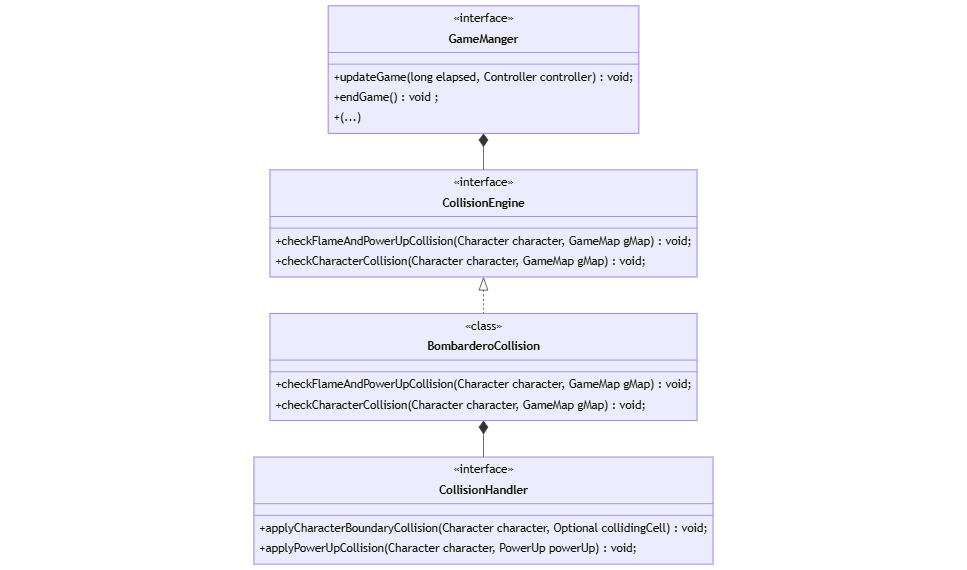
\includegraphics[width=\textwidth]{report-src/img/CollisionEngine.png}
\caption{Schema UML riassuntivo della classe BombarderoCollision}
\end{figure}

\par
Inoltre per gestire le collisioni il GameManager necessita di una Collision Engine ovvero una classe che gestisca le collisioni, questa viene passata come \verb|Strategia| da costruttore all'inizio di una partita. A sua volta l'implementazione utilizzata BombarderoCollision necessita di un CollisionHandler che risolva le collisioni da lei trovate, anche questa passata come \verb|Strategia| da costruttore. grazie a questa implementazione si possono creare nuovi modi per gestire le collisioni del gioco.
\subsection*{2. Problema da Risolvere}
\par
Nel gioco alcuni PowerUp danno il potere ai giocatori di utilizzare delle bombe che hanno effetti diversi come poter perforare i muri o esplodere da remoto

\begin{figure}[H]
\centering{}
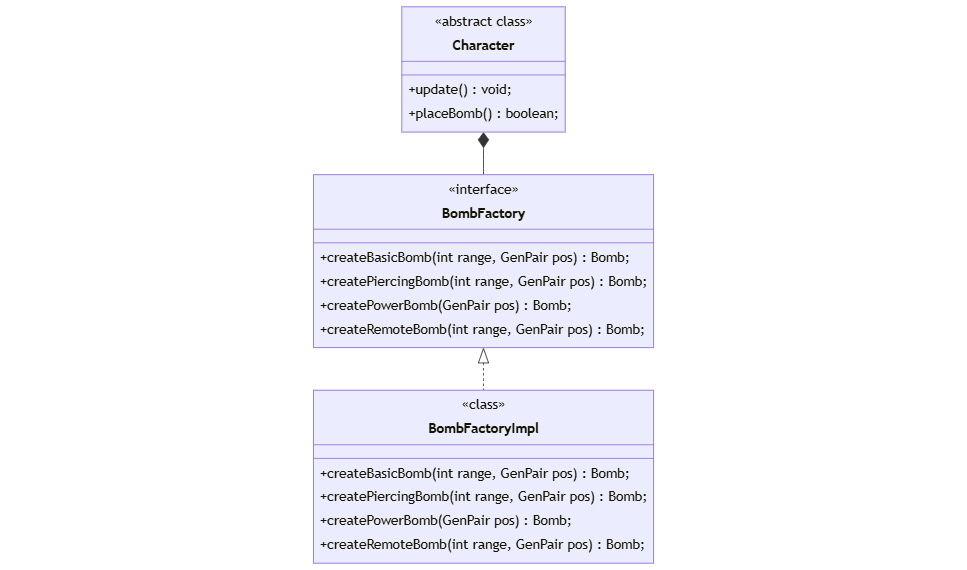
\includegraphics[width=\textwidth]{report-src/img/bombFactory.png}
\caption{Schema UML riassuntivo della classe BombFactoryImpl}
\end{figure}

\subsection*{2. Soluzione Proposta}
\par
Per la creazione delle bombe viene utilizzata una BombFactory ovvero una classe che segue il pattern \verb|Symple Factory| per cui con ogni suo metodo restituisce una Bomb con caratteristiche diverse.tutti Character che sono in gioco quando creati richiedono una BombFactory alla quale quando, dovranno piazzare delle bombe, chiederanno la Bomb equivalente al PowerUp che hanno preso. Anche in questo caso l'utilizzo del pattern \verb|Strategy| rende possibile una nuova implementazione di BombFactory.  L'implementazione delle diverse Bomb nella classe BombfactoryImpl viene fatta a partire dalla abtract class BasicBomb, sfruttando al massimo il riutilizzo del codice.


\subsection*{2. Alternativa Considerata}
\par
Nei metodi della BombFactoryImpl inizialmente era stato pensato l'utilizzo del pattern \verb|Decorator| in alternativa all'implementazione delle Bomb a partire da una classe astratta per dare la possibilita di avere bombe con piu effetti (per esempio una bomba che perfori i muri e venga fatta esplodere da remoto), questa modalità è stata scartata quando il gruppo ha deciso di tenere fede al gioco originale e non lasciare la possibilita di mescolare i tipi di bomba.

\subsection{Jacopo Turchi}


\subsubsection{Creazione dei PowerUp}
\begin{figure}[H]
\centering{}
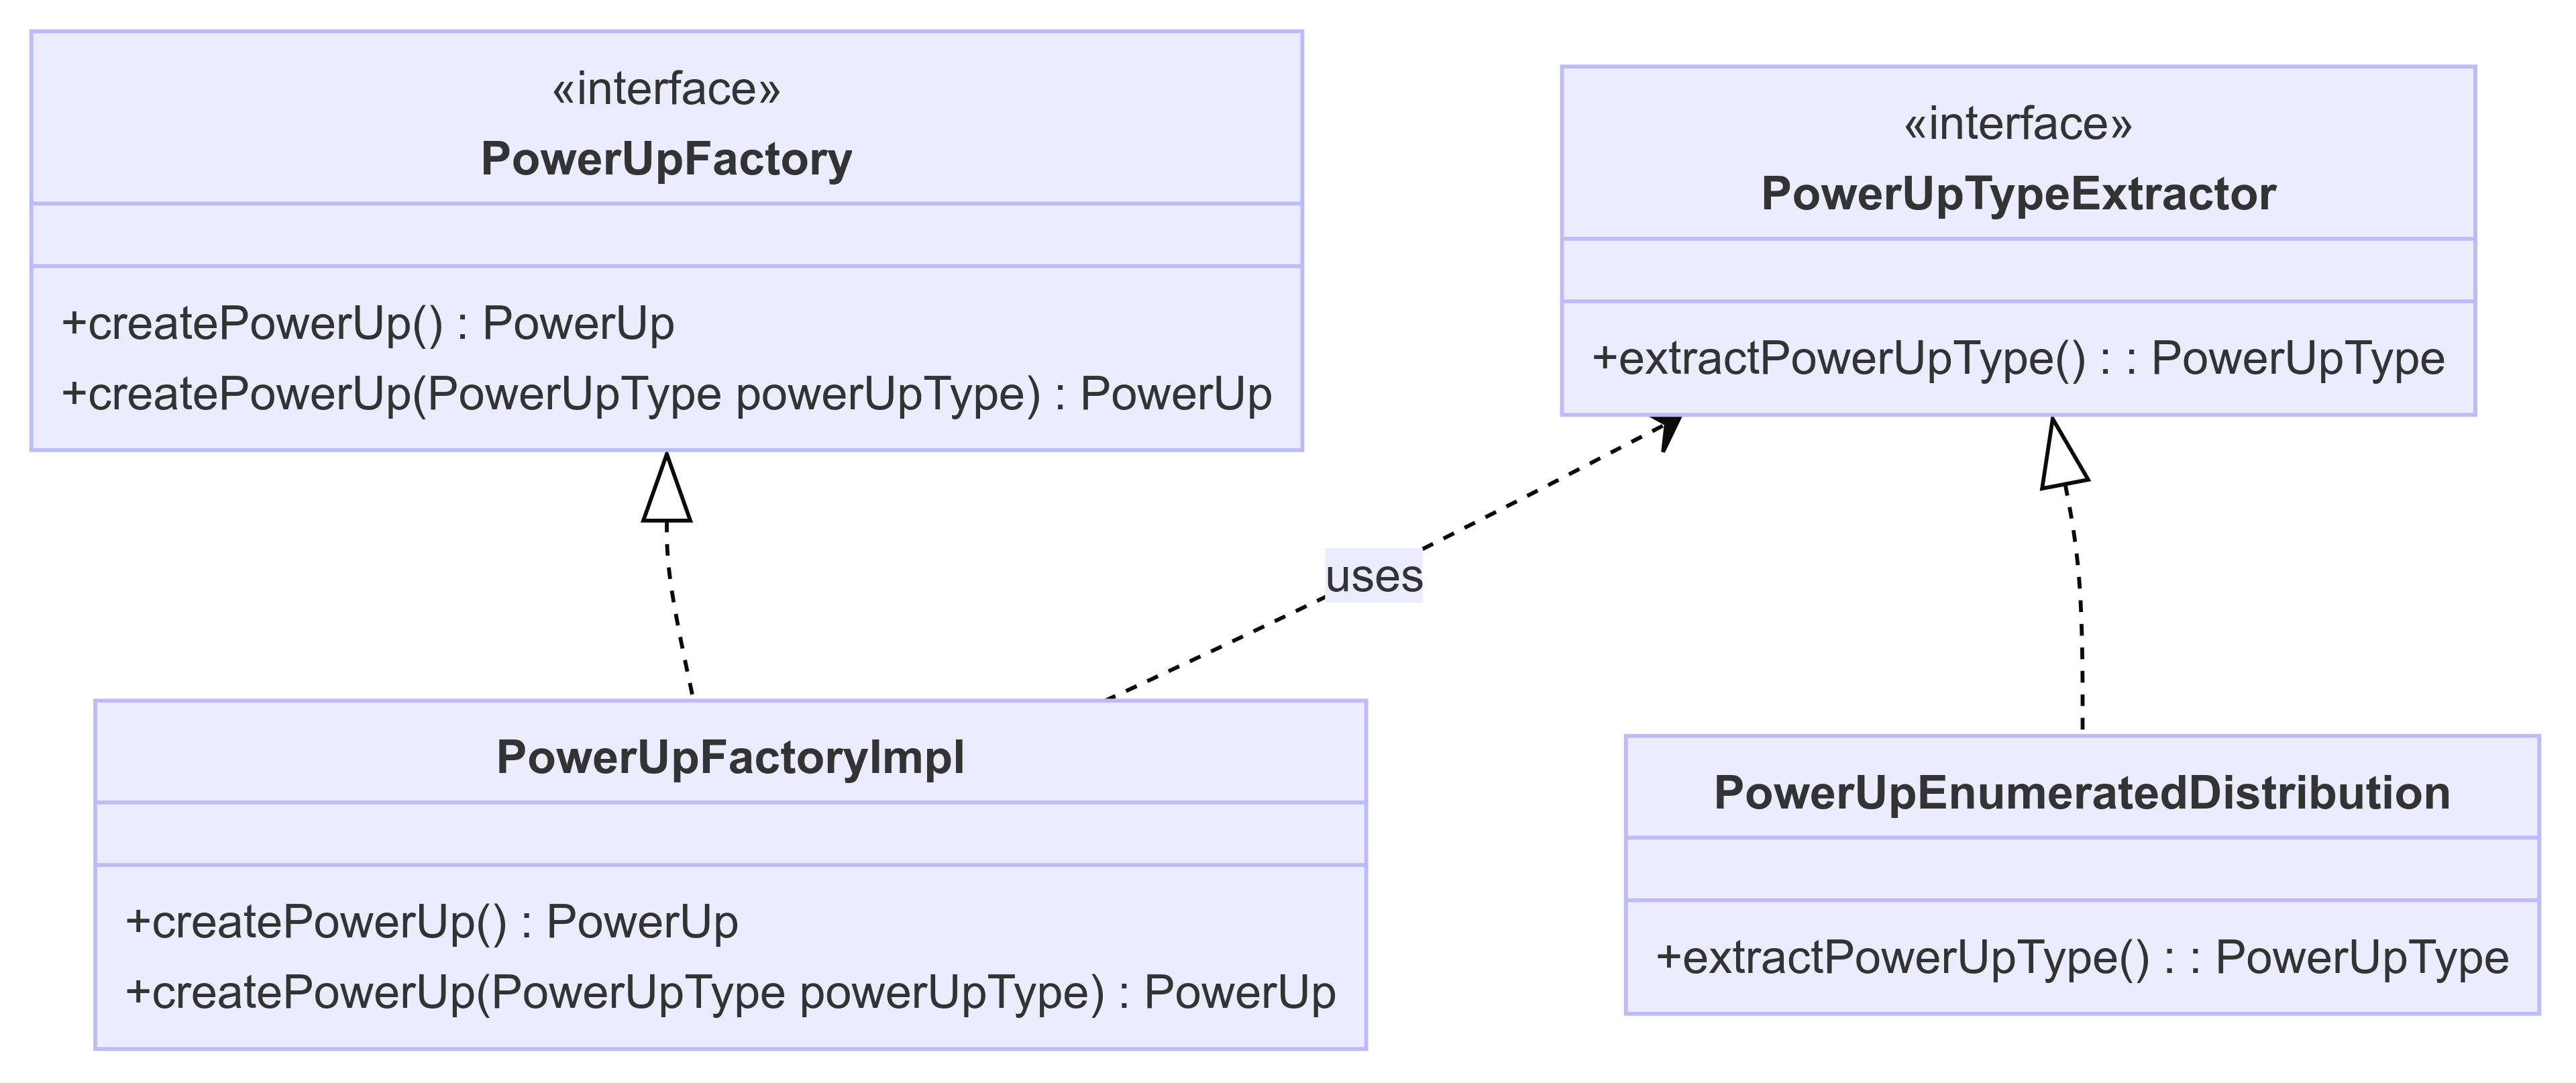
\includegraphics[width=1.0\columnwidth]{img/power-up-factory-uml.png}
\caption{Schema UML della \texttt{PowerUpFactory} e della sua implementazione}
\label{img:uml-power-up-factory}
\end{figure}
\paragraph{Problema:} I \texttt{PowerUp} devono essere generati a seguito della rottura di un \texttt{BreackableWall} in base alla loro rarità. Bisogna sviluppare una soluzione intelligente che permetta di creare PowerUp diversi.
\paragraph{Soluzione:} Seguendo il pattern \textit{Method Factory}, come da
\Cref{img:uml-power-up-factory} rispettiamo i principi SRP, OCP e DIP, dato che potenzialmente possono essere aggiunti nuovi PowerUp senza modificare il codice esistente, ma aggiungendone solo. Inoltre la factory ha il solo compito di creare i PowerUp e non dipende da implementazioni, ma dall'interfaccia.

\subsubsection{Gestione degli effetti dei PowerUp}
\begin{figure}[H]
\centering{}
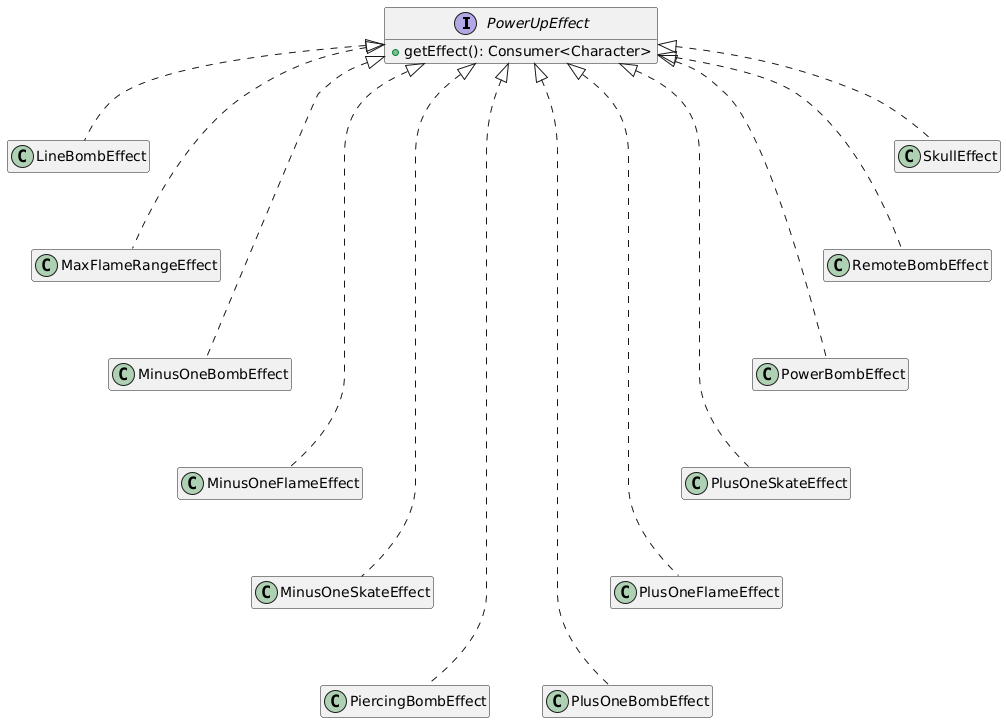
\includegraphics[width=1.0\columnwidth]{img/power-up-effect-strategy-uml.png}
\caption{Schema UML del pattern Strategy per gli effetti dei \texttt{PowerUp}}
\label{img:uml-power-up-effect-strategy}
\end{figure}
\paragraph{Problema:} I \texttt{PowerUp} sono caratterizzati da un \texttt{PowerUpEffect} che stabilisce l'effetto da applicare al \texttt{Character}. Questo effetto notiamo che deve essere intercambiabile ed è quindi necessario pensare a come incapsularne la logica.
\paragraph{Soluzione:} Seguendo il pattern \textit{Strategy}, come da
\Cref{img:uml-power-up-effect-strategy} abbiamo l'interfaccia \texttt{PowerUpEffect} che rappresenta la strategia da implementare con tutte le sue implementazioni. Con questa soluzione rispettiamo i principi SRP e OCP, dato che potenzialmente possono essere aggiunti nuovi effetti senza modificare il codice esistente (come l'abilità di passare attraverso i muri).
\paragraph{Alternativa considerata:} Un'altra alternativa valutata all'inizio era quella di inserire la responsabilità della creazione degli effetti nella \texttt{PowerUpFactory}, soluzione scartata per alleggerire la Factory e rispettare il SRP.

\subsubsection{Riuso del codice di Character}
\begin{figure}[H]
\centering{}
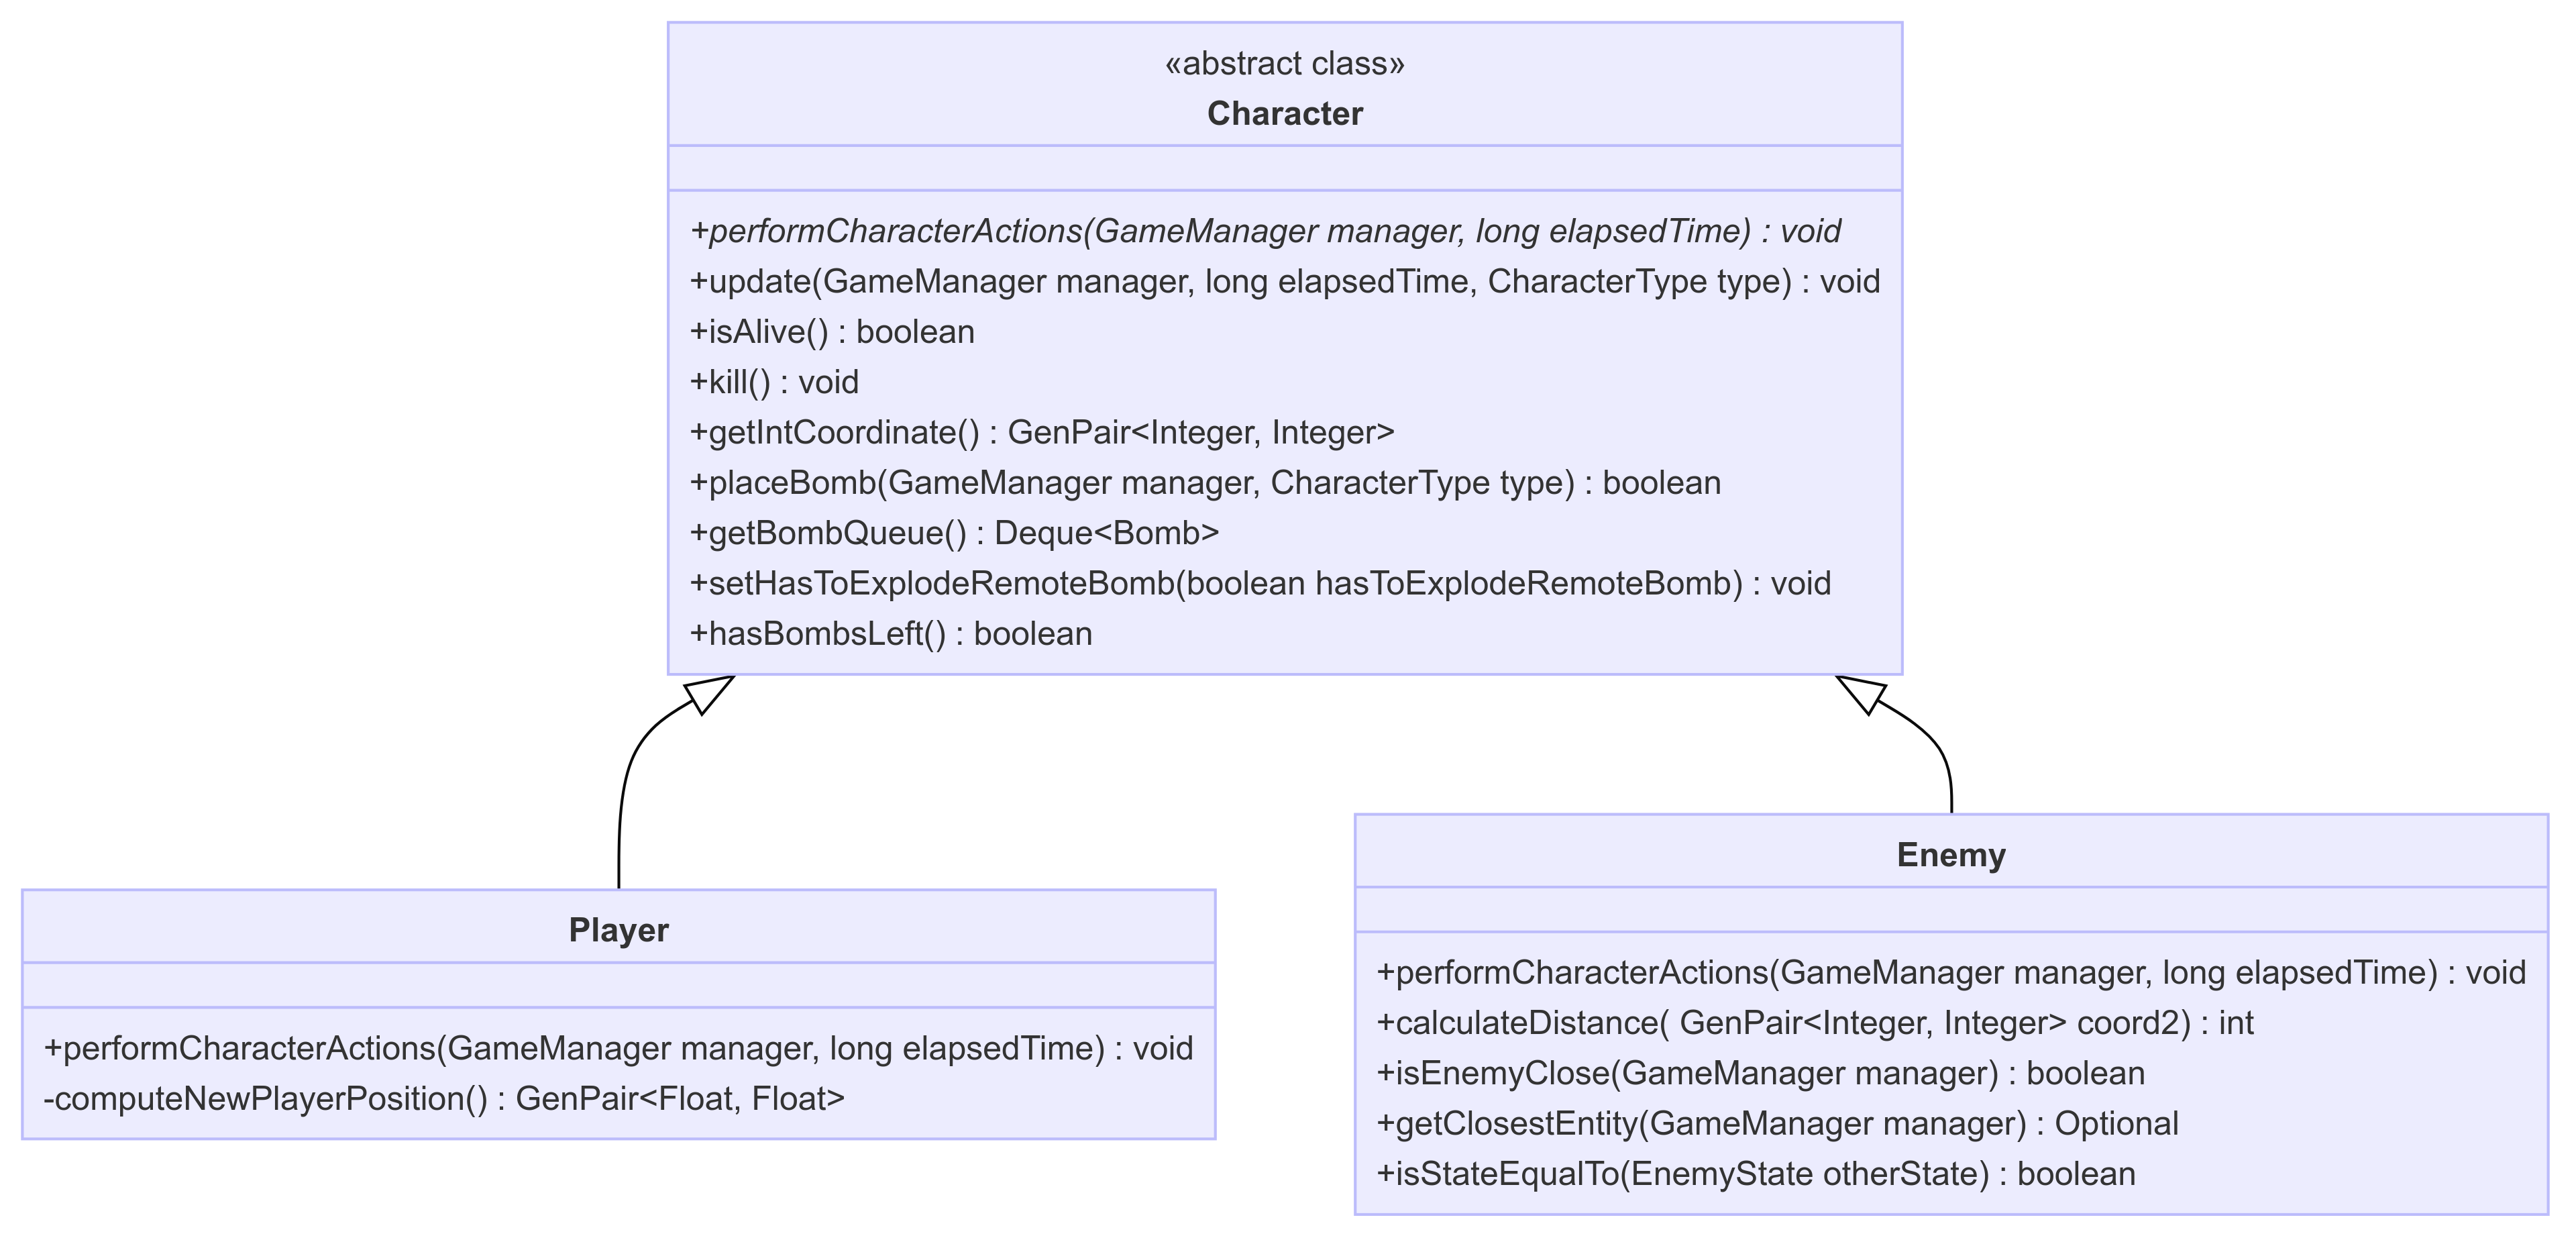
\includegraphics[width=1.0\columnwidth]{img/character-template-method-uml.png}
\caption{Schema UML dell’applicazione del pattern \textit{Template Method} per il riuso del codice di \texttt{Character}}
\label{img:uml-character-template-method}
\end{figure}
\paragraph{Problema:} Sono presenti due personaggi nel gioco, il \texttt{Player} e gli \texttt{Enemy}. E' facile notare che sono caratterizzati da molti metodi uguali portando a duplicazione di codice.
\paragraph{Soluzione:} Seguendo il pattern \textit{Template Method}, come da
\Cref{img:uml-character-template-method} abbiamo la classe astratta \texttt{Character} che con il suo template method \textit{update} detta i passi da implementare nelle sue sotto-classi. In particolare esse devono implementare il metodo astratto \texttt{performCharacterActions}. Con questa soluzione sfruttiamo il pattern insieme all'uso dell'ereditarietà per diminuire la dublicazione di codice e massimizzare il riuso.
\paragraph{Alternativa considerata:} Un'altra alternativa valutata all'inizio era quella di sfruttare la composizione per andare a definire dei manager che gestissero certe parti del \texttt{Character} come il movimento e il piazzamento di bombe (movementManager e bombManager). Tale soluzione è stata scartata in quanto si voleva evitare di complicare inutilmente la struttura e avere codice meno leggibile soprattutto in caso di chiamata da classi esterne.


\subsection{Daniele Merighi}

\par
Bomberman, come descritto precedentemente, è un gioco a tema labirintico, dove la mappa è una griglia. E’ naturale che la maggior parte dei problemi derivino dall'esplorazione dell’arena e di conseguenza dei suoi percorsi. L’obiettivo principale del nemico, però, è rimanere l’ultimo giocatore in vita. Per arrivare a ciò, bisogna che l’agent sia in grado di muoversi per la mappa, piazzare bombe in maniera consapevole, raccogliere potenziamenti per avvantaggiarsi sugli avversari e altro ancora. Essendo il tutto molto complesso, ci si è focalizzati sul riuscire a creare un nemico che abbia funzioni di base, che siano però versatili e pronte all’espansione. Di seguito si introduce lo schema UML generico, che verrà successivamente analizzato nelle sue singole parti.

\begin{figure}[h]
\centering{}
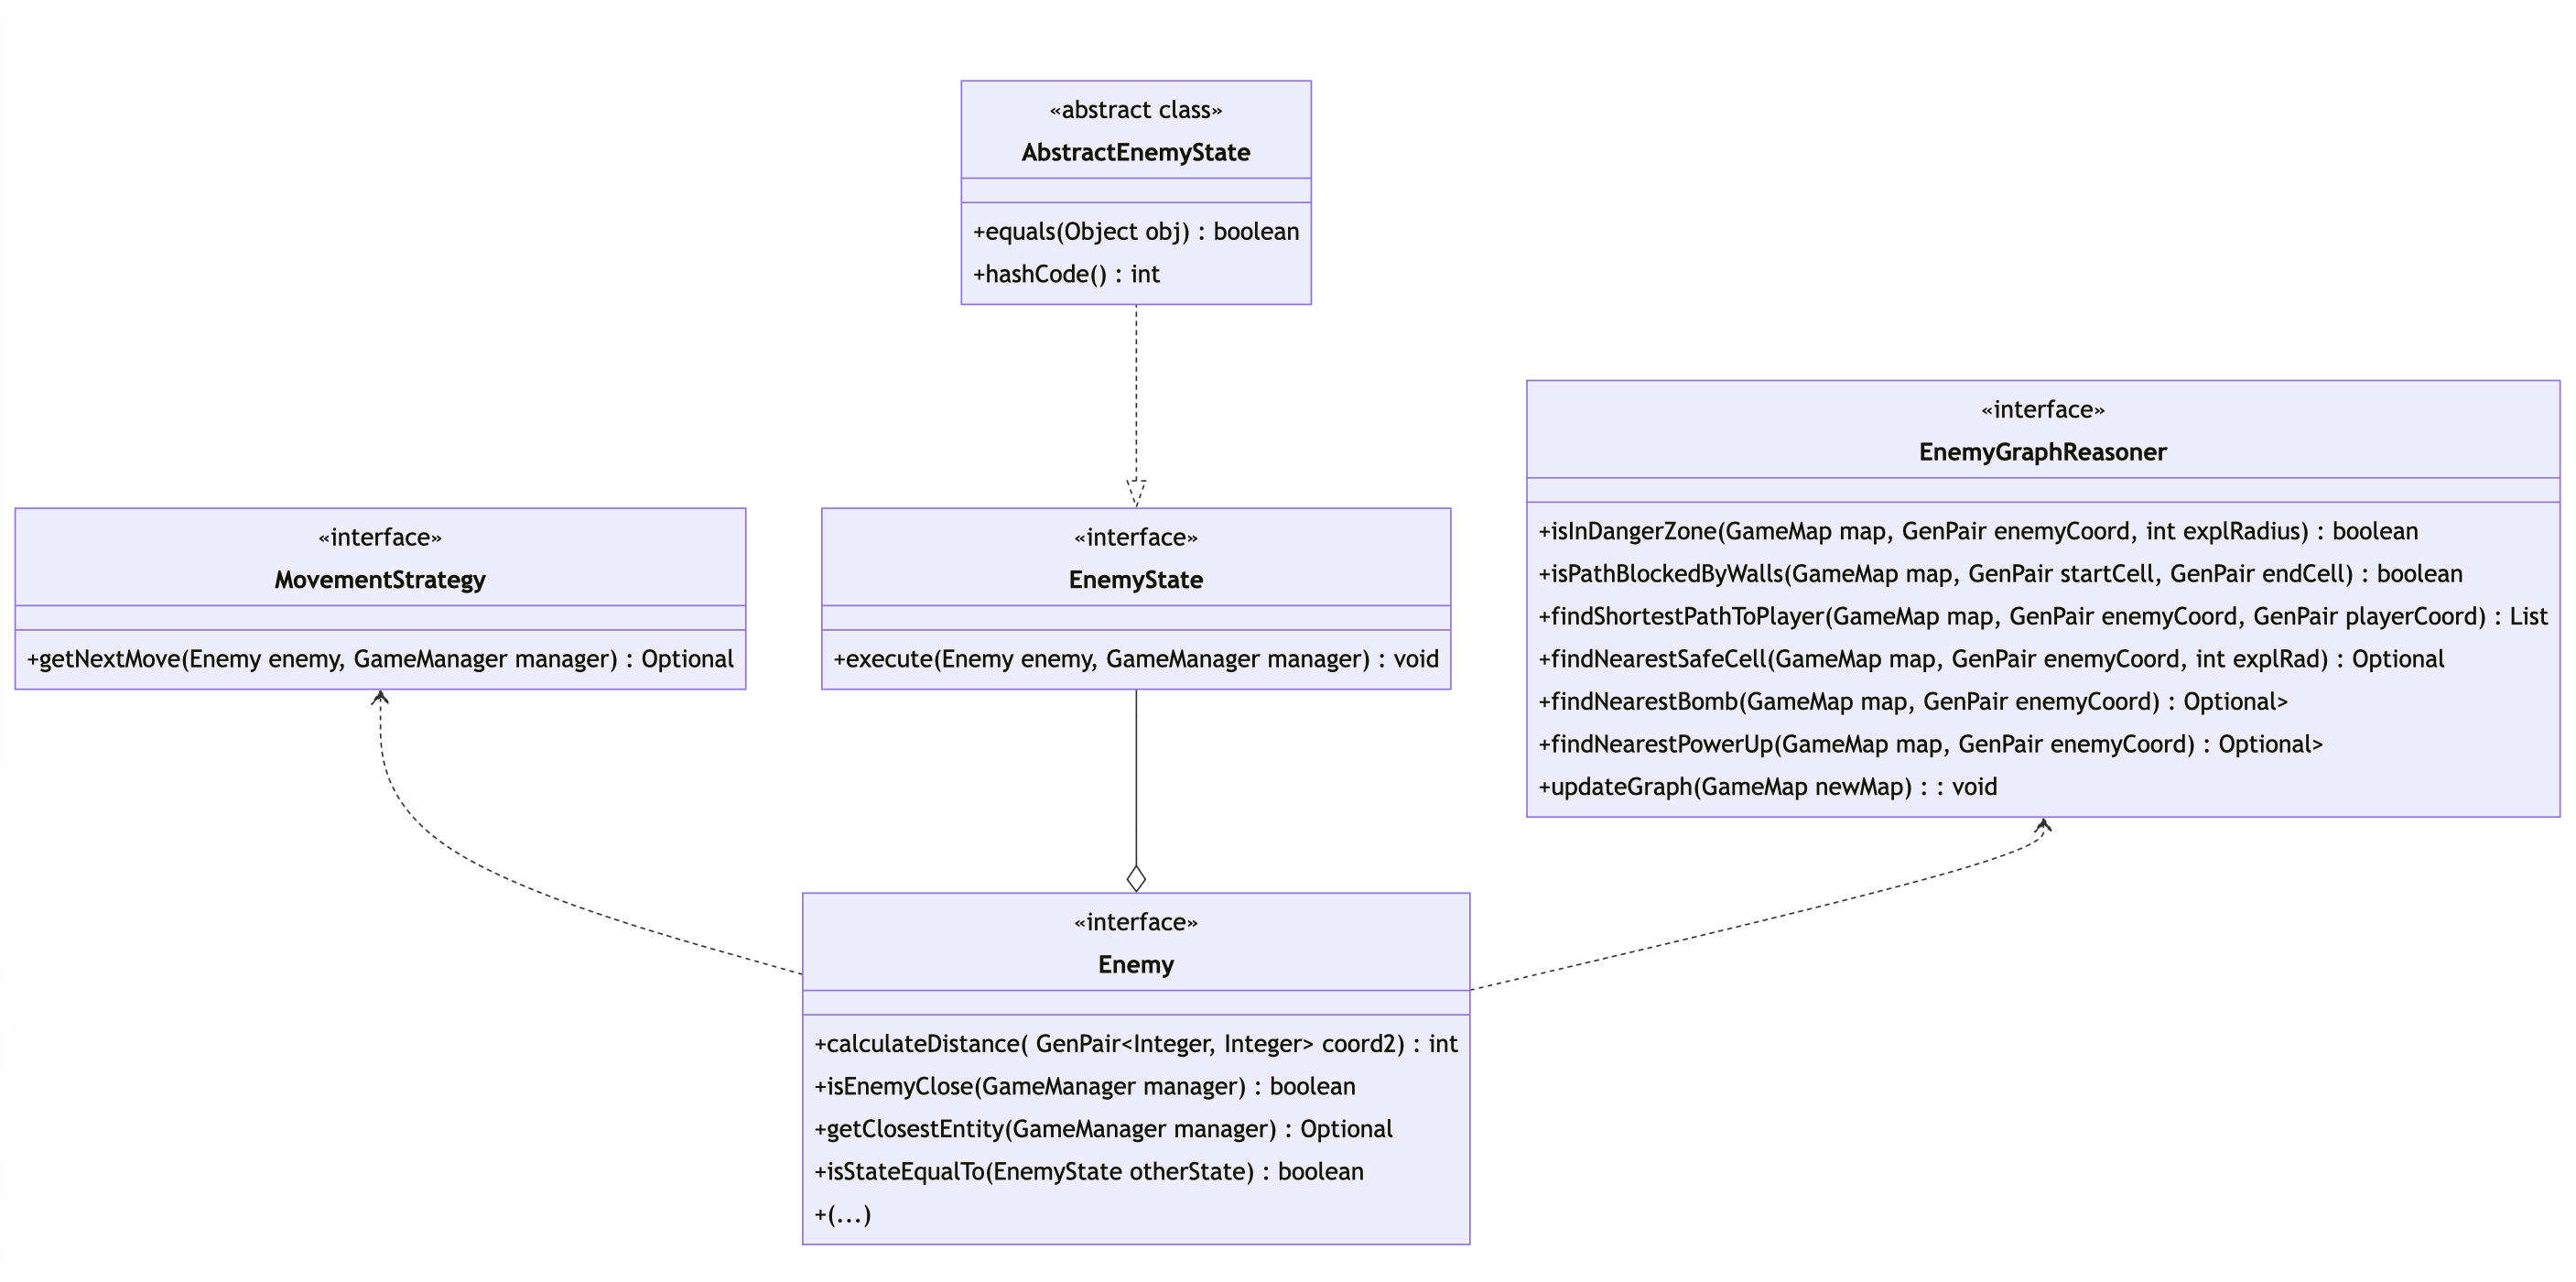
\includegraphics[width=\textwidth]{img/enemyGenerics.png}
\caption{Schema UML riassuntivo della classe Enemy}
\end{figure}

\subsection*{1. Problema da Risolvere}
\par
Uno dei problemi principali quando si gestisce il comportamento di un nemico (classe Enemy) in un videogioco è il modo in cui prende decisioni in tempo reale in base all'ambiente circostante. L’avversario deve tenere conto di numerosi ostacoli e pericoli per potersi muovere in sicurezza per la mappa di gioco. Il suo comportamento deve adattarsi continuamente alla situazione che gli si propone, deve inoltre essere flessibile e facilmente espandibile. 

\subsection*{1. Soluzione Proposta}
Per risolvere il problema, sono stati utilizzati diversi pattern di programmazione noti per strutturare il comportamento dell'Enemy. I principali utilizzati sono i seguenti:
\begin{itemize}
 \item \textbf{State Pattern:} utilizzato per rappresentare i vari stati del nemico (WAITING, ESCAPE, EXPLORING, PATROL, CHASE). Ogni stato decide cosa è meglio per l’entità in quel preciso momento e può transitare ad altri stati in base a determinate condizioni.
 \item \textbf{Strategy Pattern:} utilizzato per incapsulare diverse strategie di movimento del nemico. Questo permette di cambiare la logica senza modificare il codice stesso dell’entità.
\end{itemize}

\subsection*{1. Alternativa Considerata}
\par
Un'alternativa presa in considerazione era l'uso di una macchina a stati finiti (FSM) al posto dello State Pattern. Tuttavia, questa soluzione avrebbe reso il codice meno modulare e più difficile da estendere.

\par
Il nemico utilizza il pattern State, come illustrato in figura, per gestire i diversi comportamenti. I vari stati possono essere modificati e aggiunti e questo va ad influire sul comportamento del nemico. Durante lo sviluppo sono state definite cinque differenti "personalità" :
\begin{itemize}
 \item \textbf{Chase:} il nemico dà priorità ad inseguire l’entità a lui più vicina entro un dato raggio.
 \item \textbf{Waiting:} il nemico aspetta l’esplosione di una bomba, posizionandosi in una cella sicura.
 \item \textbf{Escape:}  il nemico cerca di raggiungere una cella sicura.
 \item \textbf{Exploring:}  il nemico raccoglie potenziamenti nelle vicinanze.
 \item \textbf{Patrol:} se il nemico non ha particolari obiettivi si muove in modo casuale.
\end{itemize}

\par
Ogni stato estende la classe AbstractEnemyState, progettata per ridurre la ridondanza di codice, la quale implementa l’interfaccia EnemyState, che rappresenta lo stato generico.

\begin{figure}[h]
\centering{}
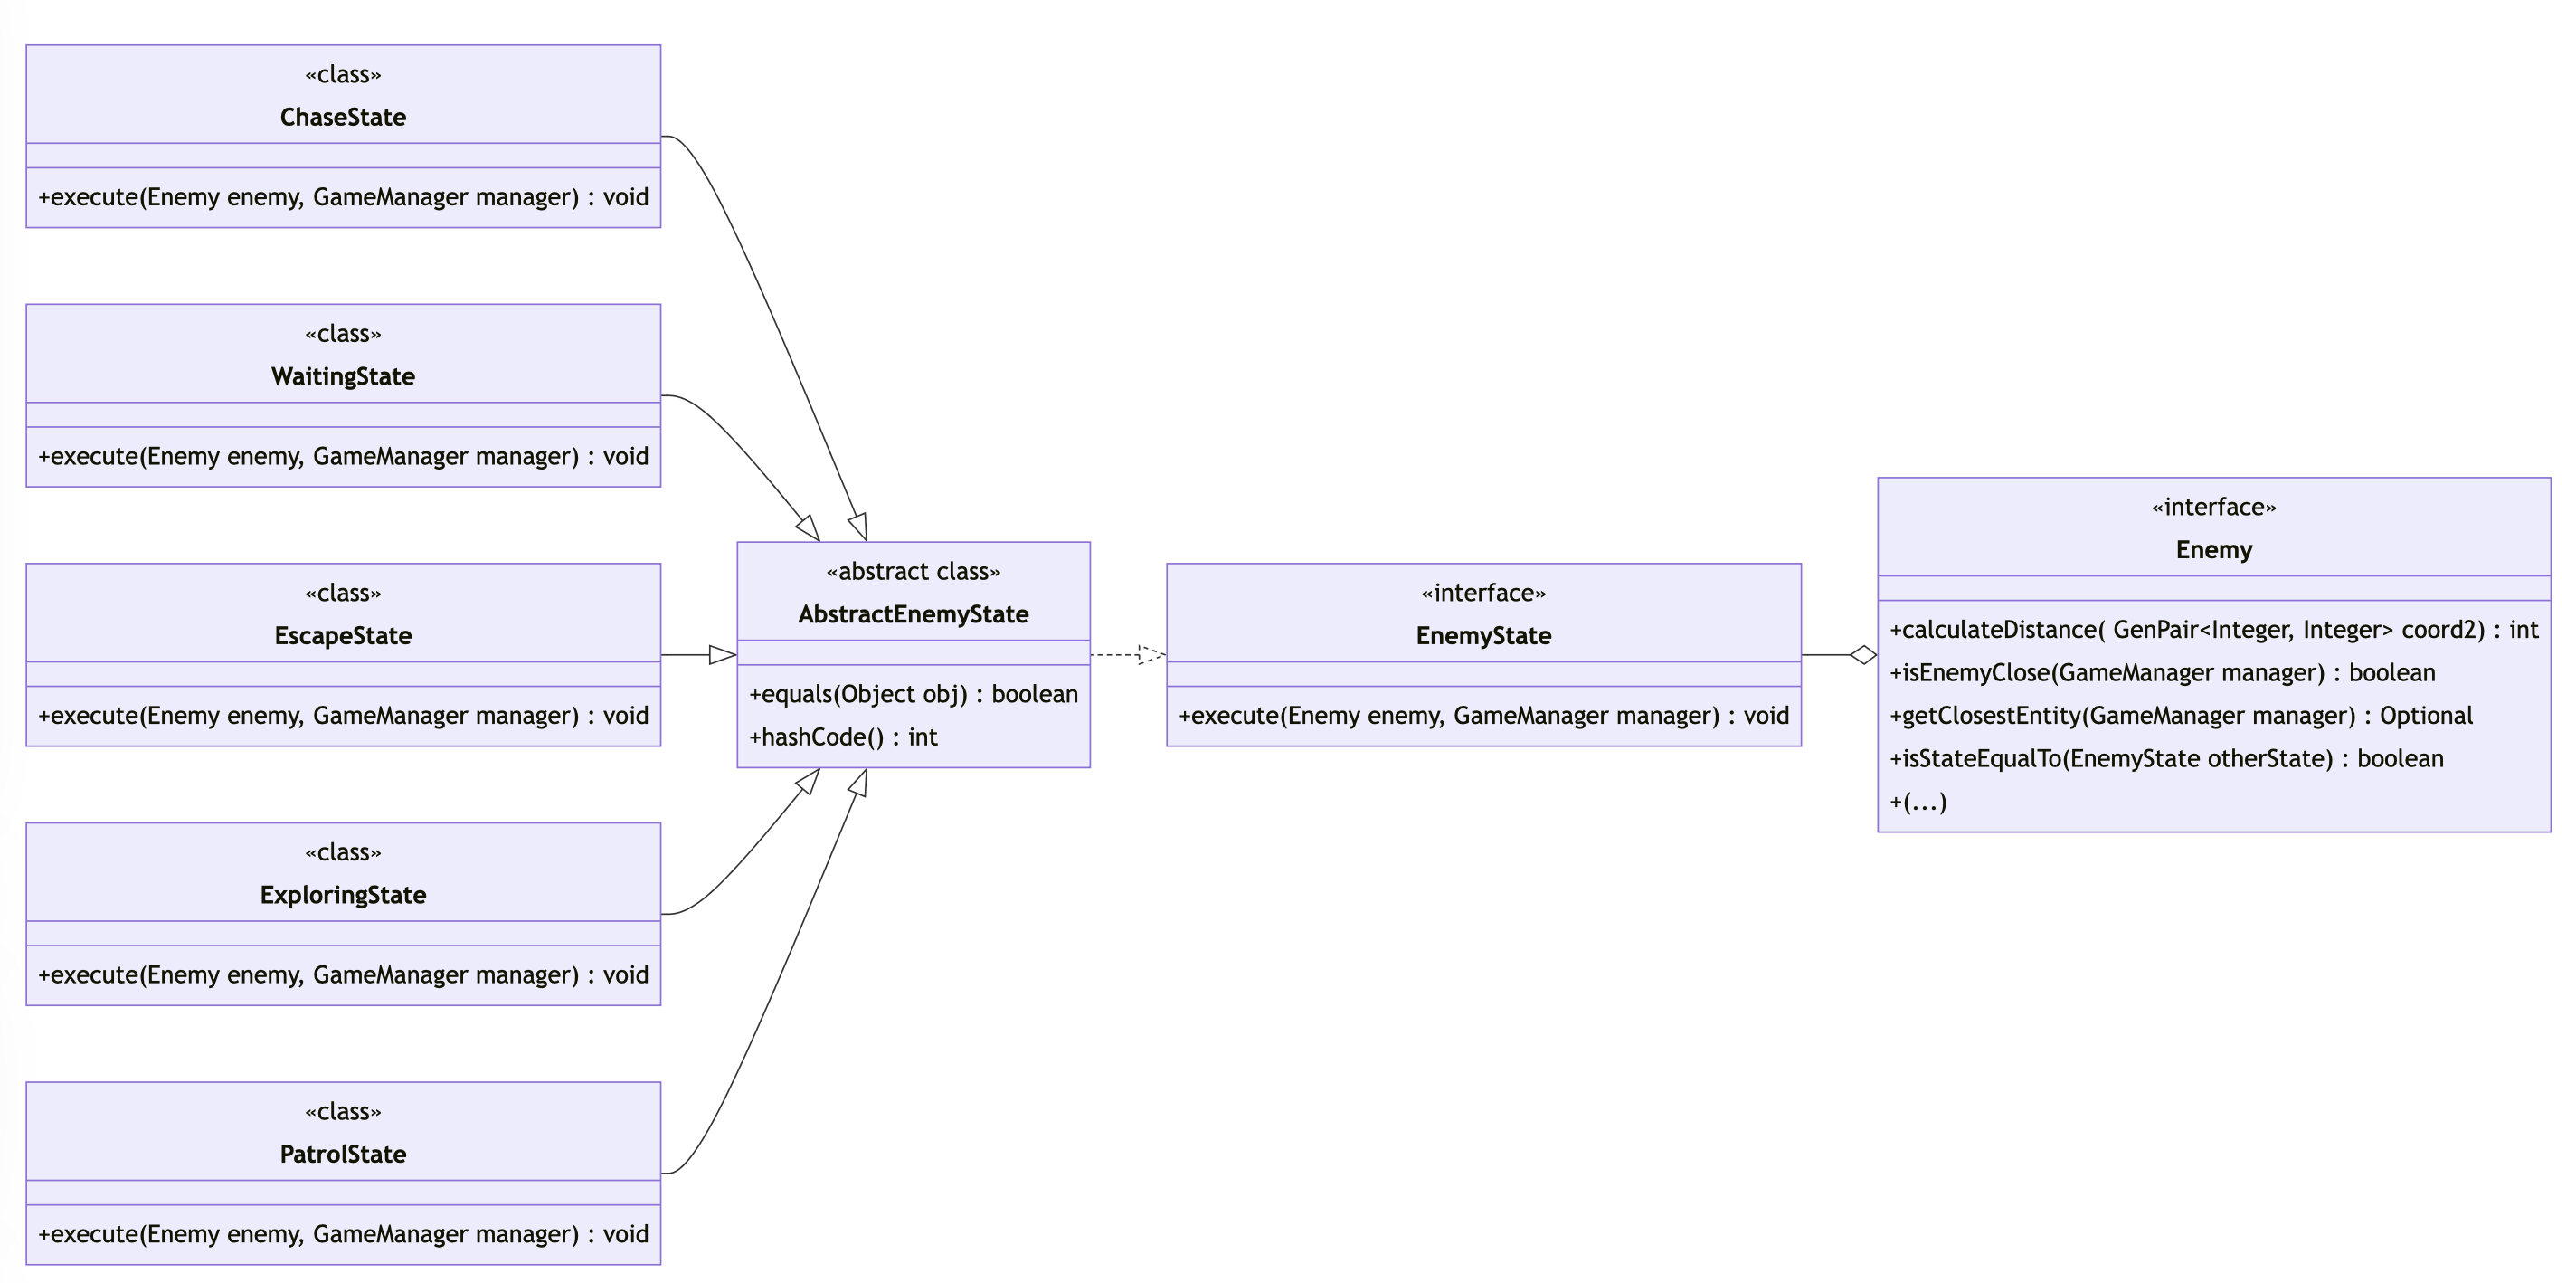
\includegraphics[width=\textwidth]{img/enemyState.png}
\caption{Schema UML che rappresenta i vari State dell'Enemy}
\end{figure}

\par
Il nemico utilizza anche il pattern Strategy, come illustrato in figura, per determinare i movimenti all’interno della mappa di gioco. Questo design permette di aggiungere in futuro strategie di movimento più sofisticate, come l’attacco e la difesa, permettendo così di rendere il comportamento del nemico più dinamico e imprevedibile. Durante la fase di sviluppo sono state realizzate diverse strategie di movimento, ognuna con un suo comportamento specifico: 
\begin{itemize}
 \item \textbf{ChaseMovementStrategy:} viene restituita la casella più vicina per raggiungere l’entità desiderata.
 \item \textbf{RandomMovementStrategy:} viene restituita una cella casuale adiacente.
 \item \textbf{EscapeMovementStrategy:} viene restituita, se esiste, la cella sicura più vicina a lui.
 \item \textbf{ExploreMovementStrategy:} viene restituito la posizione di un potenziamento a lui vicino.
 \item \textbf{ShortestMovementStrategy:} data una cella target, ti restituisce le celle che compongono il percorso minimo.
\end{itemize}

\par
L'interfaccia MovementStrategy definisce il contratto per calcolare il prossimo movimento di un nemico. Ogni classe che implementa questa interfaccia fornisce una diversa logica di movimento. 

\begin{figure}[h]
\centering{}
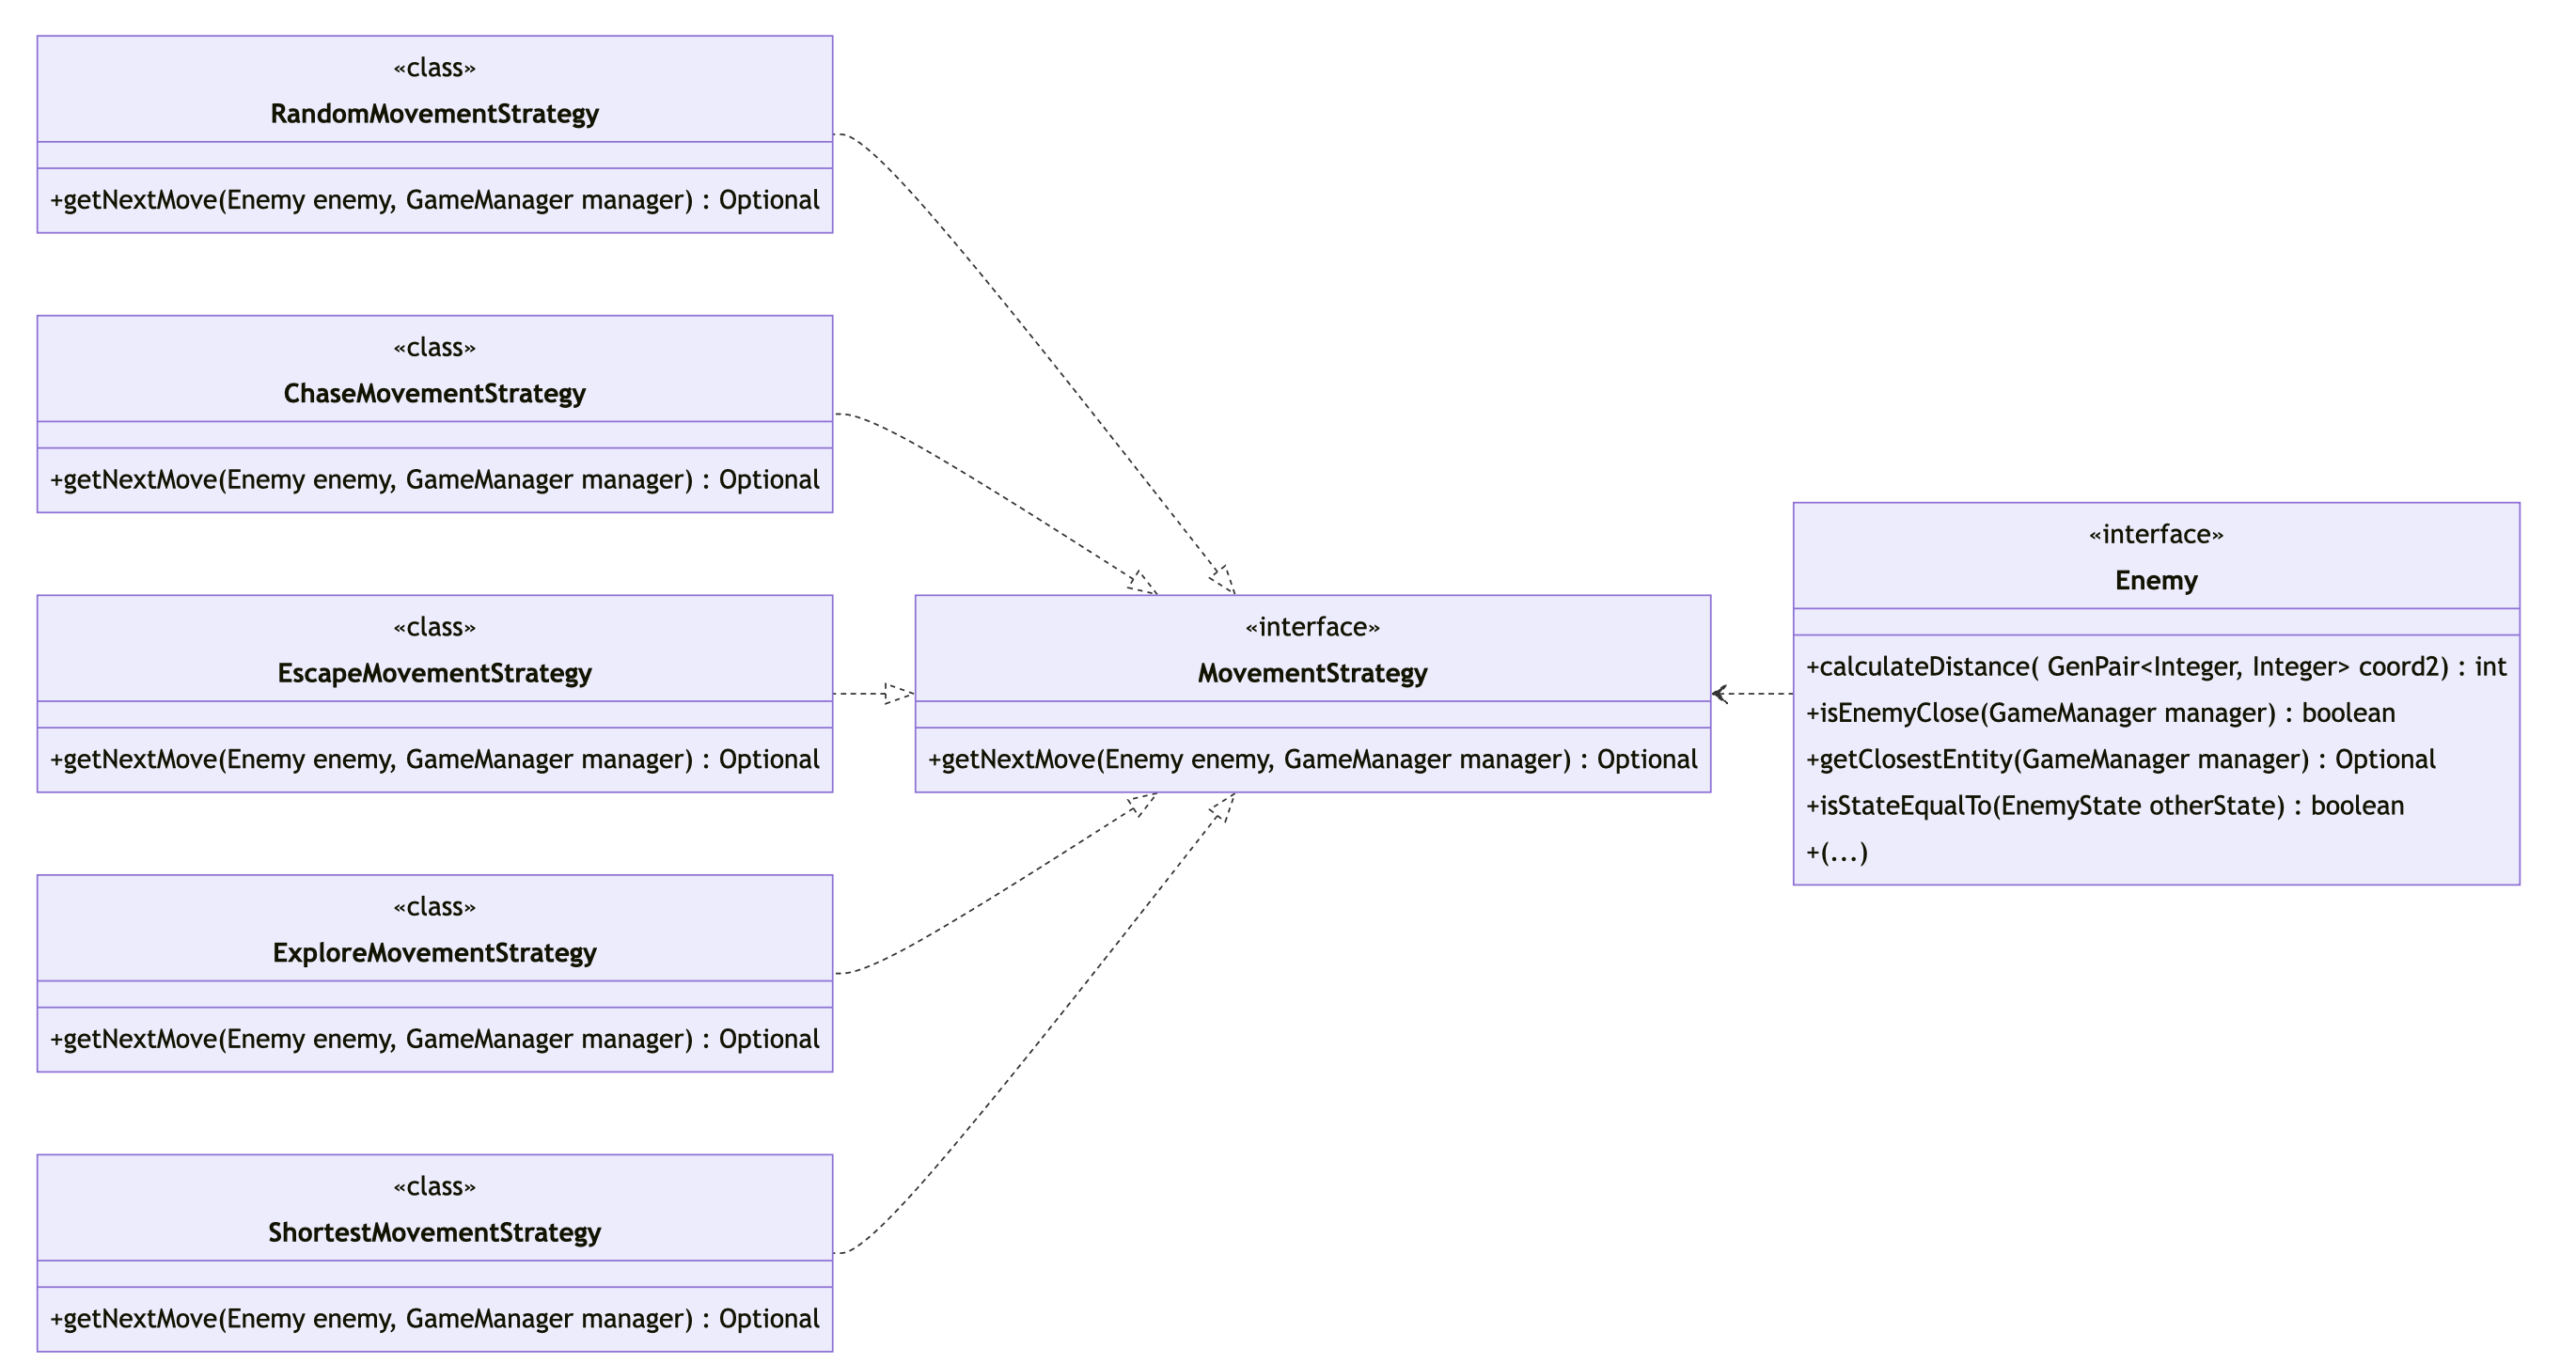
\includegraphics[width=\textwidth]{img/enemyMovement.png}
\caption{Schema UML che rappresenta i vari Movement dell'Enemy}
\end{figure}

\subsection*{2. Problema da Risolvere}
\par
Un aspetto fondamentale dei giochi “labirintici” come Bomberman è trovare il percorso migliore da un punto A ad un punto B. Quindi, dato un grafo G=(V,E) e un vertice sorgente s si ha bisogno di una strategia per esplorare sistematicamente gli archi di G per trovare il percorso raggiungibile da s che meglio si adatta alla nostra situazione. 

\subsection*{2. Soluzione Proposta}
\par
Per risolvere il problema si è deciso di trasformare la mappa di gioco da un dizionario (che associa ad ogni coordinata (x,y) una cella) ad un grafo.
La classe che gestisce ciò è GraphBuilderImpl, definita statica, dove ogni cella della mappa (tranne i muri indistruttibili) viene vista come un nodo. Questi sono collegati tra loro da archi pesati, che rappresentano un cammino che il nemico può compiere, da il nodo di origine a quello di destinazione. Solo le celle tra loro adiacenti vengono quindi collegate da un arco. Il suo costo può essere di due tipi:
\begin{itemize}
    \item da muro distruttibile a ogni altro nodo: costo 2.5
    \item ogni altro collegamento: costo 1
\end{itemize}
Questa decisione è stata presa per dare maggiore importanza ai percorsi già disponibili nella mappa, invece che crearne di nuovi. Questo favorisce anche il percorso di inseguimento da parte del nemico quando vede un'altra entità.

\par
Una volta definito il grafo, sono state scelte due tipologie di algoritmi per la sua esplorazione:
\begin{itemize}
    \item \textbf{Breadth-First Search (BFS):} questa produce un albero con nodo radice s che contiene tutti i vertici raggiungibili. Per ogni vertice v raggiungibile da s, il cammino semplice nell’albero prodotto dalla BFS da s a v, corrisponde ad un cammino minimo da s a v in G.
    \item \textbf{Dijkstra:} questo trova il percorso minimo da un nodo sorgente a tutti gli altri nodi in un grafo aciclico e con pesi non negativi.
\end{itemize}

\begin{figure}[h]
\centering{}
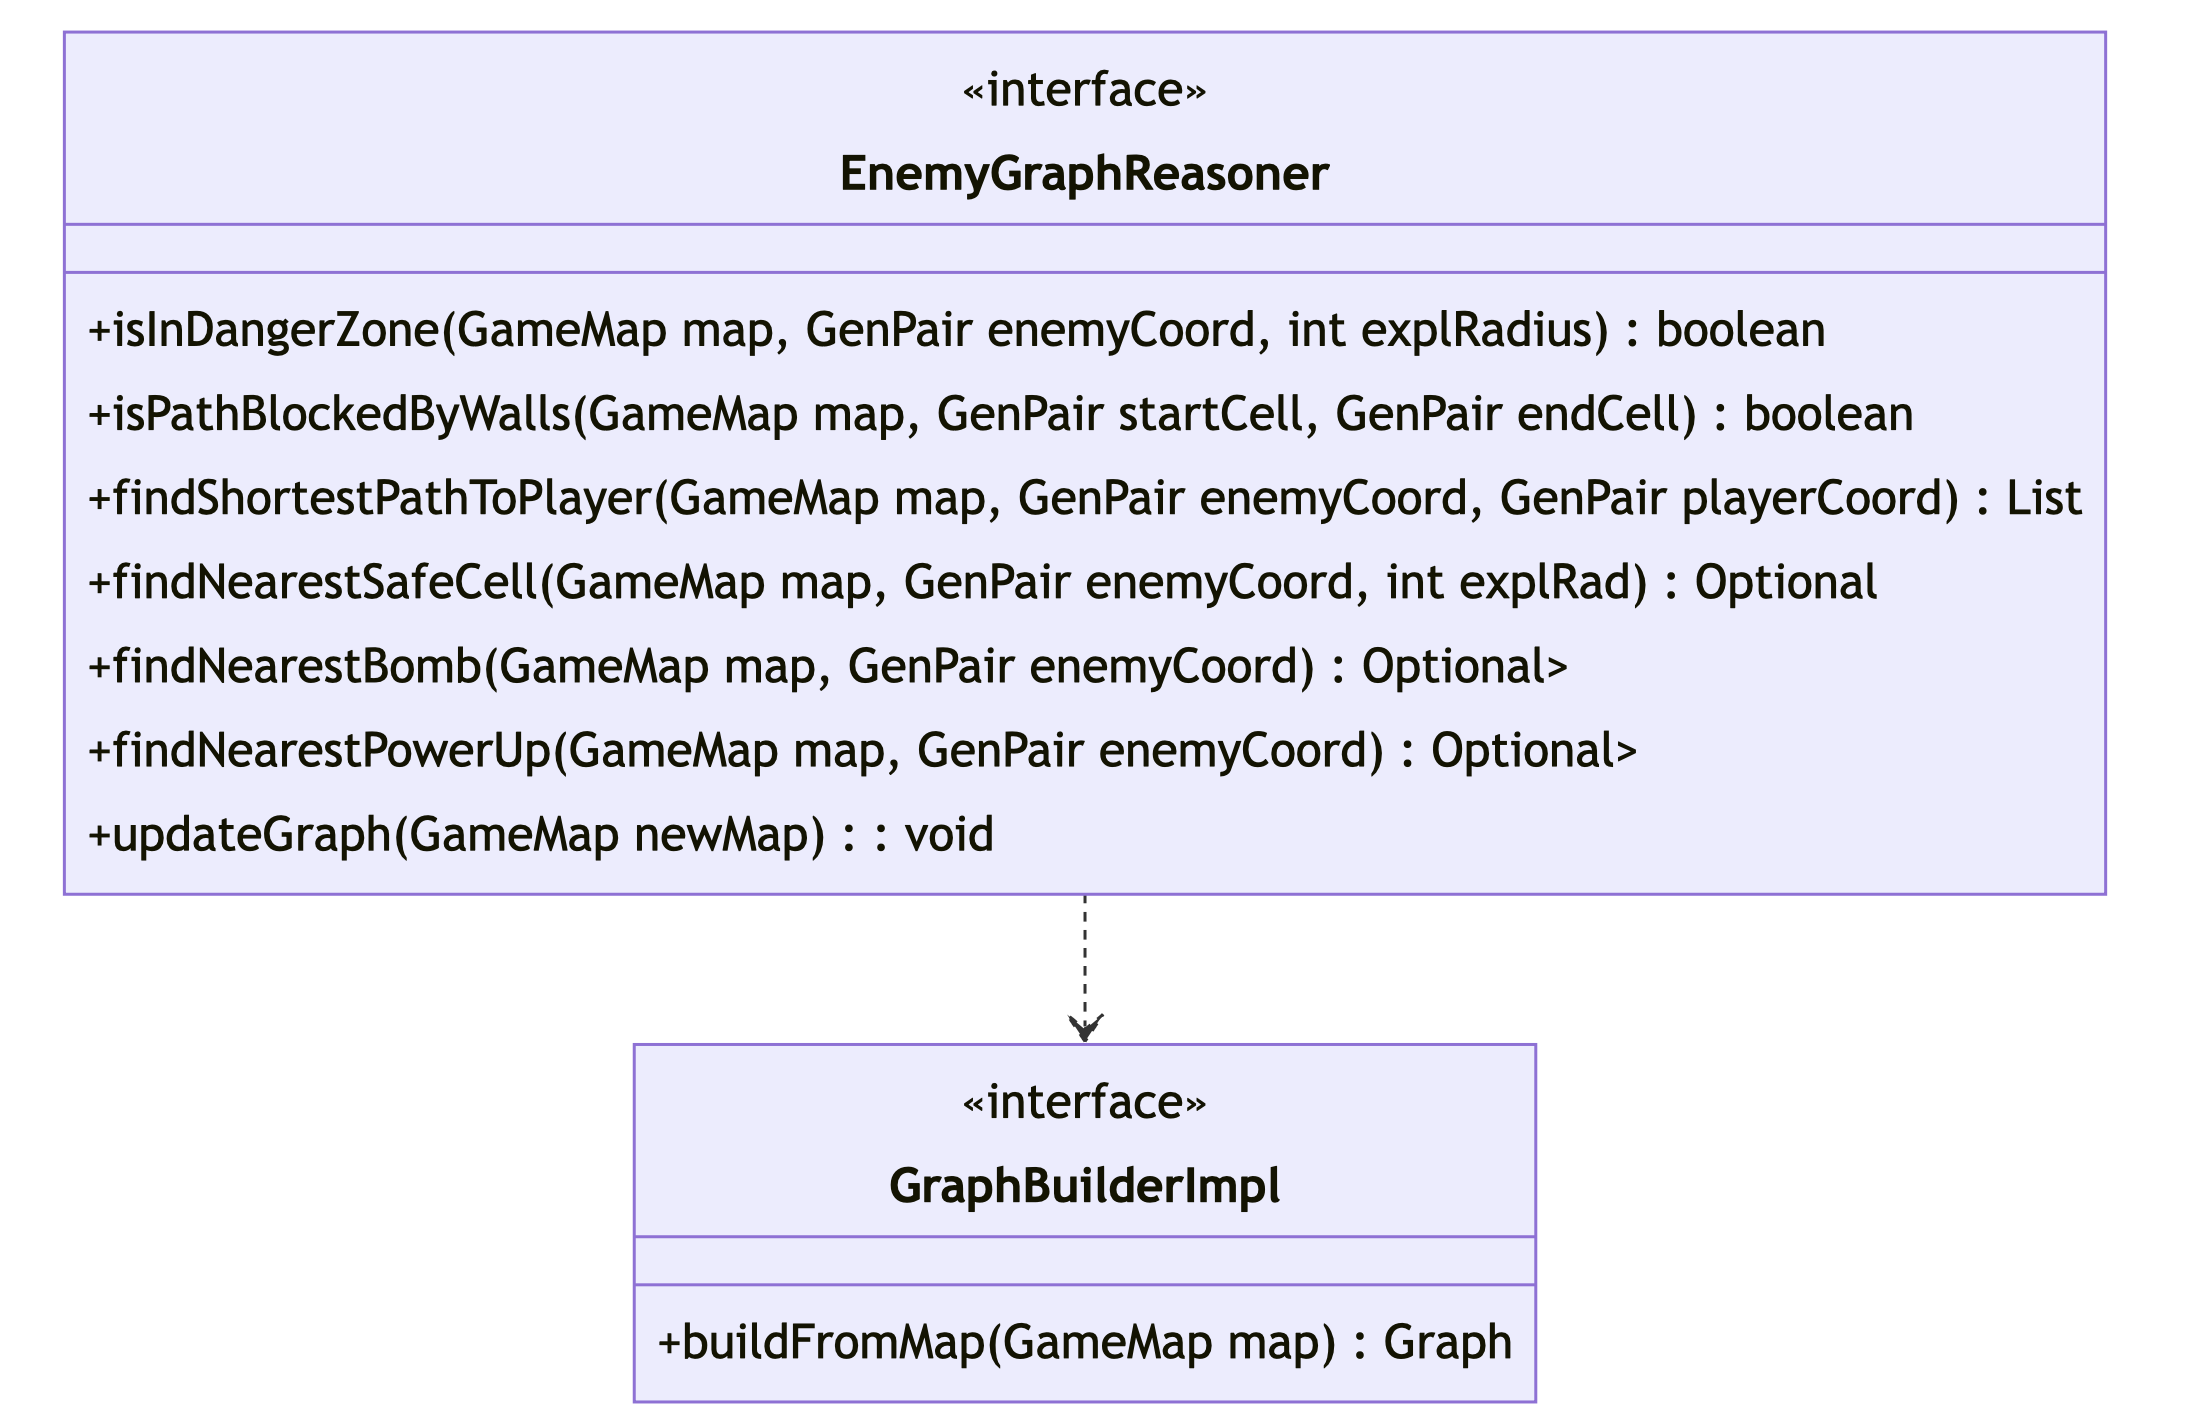
\includegraphics[width=\textwidth]{img/enemyGraph.png}
\caption{Schema UML che rappresenta la classe del Grafo}
\end{figure}

\chapter{Sviluppo}
\section{Testing automatizzato}

\par
La classe \texttt{TestGraphBuilder} verifica la corretta creazione del grafo a partire dalla mappa di gioco. Di seguito sono descritti i principali casi di test:
\begin{itemize}
    \item verifica delle dimensioni della mappa vuota (con solo muri indistruttibili)
    \item verifica delle dimensioni della mappa con ostacoli
    \item verifica dei pesi degli archi nel grafo
\end{itemize}

\par
La classe \texttt{TestReasoner} testa le interrogazioni che vengono fatte al grafo. Di seguito sono descritti i principali casi di test:
\begin{itemize}
    \item verifica se una cella è in una zona di pericolo (dove sta per esplodere una bomba)
    \item verifica se tra due celle è presente un muro
    \item verifica del percorso minimo tra un nemico ed il player
    \item verifica della cella sicura più vicina al nemico dopo l’esplosione di una bomba
\end{itemize}

\par
La classe \texttt{TestEnemy} verifica il giusto comportamento del nemico al verificarsi di determinate situazioni. Di seguito sono descritti i principali casi di test:
\begin{itemize}
    \item verifica se lo stato del nemico è Patrol se il player non è in un dato raggio e di conseguenza se si muove in maniera casuale
    \item verifica se lo stato del nemico cambia a Chase quando il player è nel raggio visivo
    \item verifica se il nemico “insegue” il player quando è in Chase
    \item verifica se il nemico in presenza di una bomba cambia il suo stato a Escape, posizionandosi poi in una zona sicura
    \item verifica se il nemico posiziona una bomba se tra lui e il player è presente un muro distruttibile
\end{itemize}

\par
La classe \texttt{TestInput} verifica che la classe KeyboardInput gestisca correttamente i vari input che riceve. Di seguito sono descritti i principali casi di test:
\begin{itemize}
    \item verifica la corretta funzione dei vari tasti (ESC, SPACE, L, P, W, A, S, D)
    \item verifica il corretto funzionamento di movimenti complessi
    \item verifica la possibilità di piazzare bombe mentre il personaggio si muove
\end{itemize}

\par
La classe \texttt{TestPowerUp} verifica che la classe PowerUp e la sua corrispettiva factory funzionino. In particolare:
\begin{itemize}
    \item verifica la corretta creazione dei PowerUp
    \item verifica che lo SkullEffect funzioni correttamente
\end{itemize}

\par
La classe \texttt{TestPlayer} verifica che la classe Player e la sua classe astratta Character da cui eredita i metodi funzionino. In particolare:
\begin{itemize}
    \item verifica la capacità del player di girarsi nelle quattro direzioni possibili
    \item verifica che il movimento del player venga eseguito correttamente
    \item verifica che il player sia in grado di piazzare le bombe
\end{itemize}

\par
La classe \texttt{TestBomb} : verifica che la BombFactoryImpl e le Bomb funzionino nel modo corretto
\begin{itemize}
    \item verifica l'interazione dell'esplosione con vari tipi di Cell 
    \item verifica il corretto piazzamento dei diversi tipi di Bomb
    \item verifica gli effetti di tutti i tipi di Bomb
\end{itemize}

\par
La classe \texttt{TestCollision} : verifica le classi RectangleBoundingBox, BombarderoCollision e CollisionHandler 
\begin{itemize}
    \item verifica che le collisioni con un ostacolo siamo riscontrate in tutte e 4 le direzioni e successivamente risolte  
    \item verifica quando un personaggio si trova sopra ad una Cell di tipo Powerup o Flame
\end{itemize}
\par
per il testing specifico della risoluzione delle collisioni si è preferito fare test di persona così da poter decidere la grandezza delle BoundingBox

\section{Note di sviluppo}

\subsection{qualcosa di Federico Bagattoni}
\subsection{Luca Venturini}

\subsubsection{Utilizzo di Stream Java}
\textbf{Permalink:} \url{https://github.com/DanieleMerighi/OOP23-bombardero/blob/43c0418f98602e303e34baf20629ccd1dd0a7c1b/src/main/java/it/unibo/bombardero/bomb/impl/BasicBomb.java#L115-L140}

\subsubsection{Utilizzo di generici e Functional Interface}
\textbf{Permalink:} \url{https://github.com/DanieleMerighi/OOP23-bombardero/blob/a94a829f9745cfda90a3125da40c183ad68c571e/src/main/java/it/unibo/bombardero/map/api/GenPair.java#L46-L57}

\subsubsection{Functional Interface e Lambda expression}
\textbf{Permalink:} \url{https://github.com/DanieleMerighi/OOP23-bombardero/blob/a94a829f9745cfda90a3125da40c183ad68c571e/src/main/java/it/unibo/bombardero/map/api/Functions.java#L22-L85}

\subsection{Jacopo Turchi}

\subsubsection{Uso di lambda expression in vari punti, in particolare per la Strategy, combinato all'uso di Runnable, Method Reference e Optional}
\textbf{Permalink:} \url{https://github.com/DanieleMerighi/OOP23-bombardero/blob/43c0418f98602e303e34baf20629ccd1dd0a7c1b/src/main/java/it/unibo/bombardero/cell/powerUp/impl/SkullEffect.java#L54C9-L72C11}

\subsubsection{Uso di stream in vari punti, per esempio:}
\textbf{Permalink:} \url{https://github.com/DanieleMerighi/OOP23-bombardero/blob/43c0418f98602e303e34baf20629ccd1dd0a7c1b/src/main/java/it/unibo/bombardero/cell/powerUp/impl/PowerUpImpl.java#L41-L62}

\subsubsection{Uso di Supplier e Consumer:}
\textbf{Permalink:} \url{https://github.com/DanieleMerighi/OOP23-bombardero/blob/43c0418f98602e303e34baf20629ccd1dd0a7c1b/src/main/java/it/unibo/bombardero/cell/powerUp/impl/PowerUpFactoryImpl.java#L64C9-L68C67}
\textbf{Permalink:} \url{https://github.com/DanieleMerighi/OOP23-bombardero/blob/43c0418f98602e303e34baf20629ccd1dd0a7c1b/src/main/java/it/unibo/bombardero/cell/powerUp/impl/PowerBombEffect.java#L27C5-L29C6}

\subsubsection{Uso della libreria Apache Commons}
\textbf{Permalink:} \url{https://github.com/DanieleMerighi/OOP23-bombardero/blob/43c0418f98602e303e34baf20629ccd1dd0a7c1b/src/main/java/it/unibo/bombardero/cell/powerUp/impl/PowerUpEnumeratedDistribution.java#L25-L40}




\subsection{Daniele Merighi}
\par
\subsubsection{Utilizzo della libreria jgrapht.Graph}
Utilizzata in vari punti, un esempio è:
\url{https://github.com/DanieleMerighi/OOP23-bombardero/blob/a94a829f9745cfda90a3125da40c183ad68c571e/src/main/java/it/unibo/bombardero/character/AI/impl/GraphBuilderImpl.java#L45-L57}

\par
\subsubsection{Utilizzo della libreria jgrapht.traverse}
Permalink: \url{https://github.com/DanieleMerighi/OOP23-bombardero/blob/a94a829f9745cfda90a3125da40c183ad68c571e/src/main/java/it/unibo/bombardero/character/AI/impl/EnemyGraphReasonerImpl.java#L229-L241}

\par
\subsubsection{Utilizzo delle \texttt{Stream} Java}
Utilizzando dove è stato possibile, il seguente è un singolo esempio: 
\url{https://github.com/DanieleMerighi/OOP23-bombardero/blob/a94a829f9745cfda90a3125da40c183ad68c571e/src/main/java/it/unibo/bombardero/character/AI/impl/EnemyGraphReasonerImpl.java#L75C5-L85C6}

%
In questa sezione, \textit{dopo l'elenco},
vanno menzionati ed attributi con precisione eventuali pezzi di codice ``riadattati'' (o scopiazzati...) da Internet o da altri progetti,
pratica che tolleriamo ma che non raccomandiamo.
%
Si rammenta agli studenti che non è consentito partire da progetti esistenti e procedere per modifiche successive.
%
Si ricorda anche che i docenti hanno in mano strumenti antiplagio piuttosto raffinati e che ``capiscono'' il codice e la storia delle modifiche del progetto,
per cui tecniche banali come cambiare nomi (di classi, metodi, campi, parametri, o variabili locali),
aggiungere o togliere commenti,
oppure riordinare i membri di una classe vengono individuate senza problemi.
%
Le regole del progetto spiegano in dettaglio l'approccio dei docenti verso atti gravi come il plagiarismo.

I pattern di design \textbf{non} vanno messi qui.
%
L'uso di pattern di design (come suggerisce il nome) è un aspetto avanzato di design, non di implementazione,
e non va in questa sezione.

\subsection*{Elementi positivi}

\begin{itemize}
	\item Si elencano gli aspetti avanzati di linguaggio che sono stati impiegati
	\item Si elencano le librerie che sono state utilizzate
	\item Per ciascun elemento, si fornisce un permalink
	\item Ogni permalink fa riferimento ad uno snippet di codice scritto dall'autore della sezione (i docenti verificheranno usando \texttt{git blame})
	\item Se si è utilizzato un particolare algoritmo, se ne cita la fonte originale.
	Ad esempio, se si è usato Mersenne Twister per la generazione di numeri pseudo-random, si cita \cite{mersenne}.
	\item Si identificano parti di codice prese da altri progetti, dal web, o comunque scritte in forma originale da altre persone.
	In tal senso, si ricorda che agli ingegneri non è richiesto di re-inventare la ruota continuamente:
	se si cita debitamente la sorgente è tollerato fare uso di di snippet di codice open source per risolvere velocemente problemi non banali.
	Nel caso in cui si usino snippet di codice di qualità discutibile,
	oltre a menzionarne l'autore originale si invitano gli studenti ad adeguare tali parti di codice agli standard e allo stile del progetto.
	Contestualmente, si fa presente che è largamente meglio fare uso di una libreria che copiarsi pezzi di codice:
	qualora vi sia scelta (e tipicamente c'è), si preferisca la prima via.
\end{itemize}

\subsection*{Elementi negativi}
\begin{itemize}
	\item Si elencano feature core del linguaggio invece di quelle segnalate. Esempi di feature core da non menzionare sono:
    \begin{itemize}
        \item eccezioni;
        \item classi innestate;
        \item enumerazioni;
        \item interfacce.
    \end{itemize}
	\item Si elencano applicazioni di terze parti (peggio se per usarle occorre licenza, e lo studente ne è sprovvisto) che non c'entrano nulla con lo sviluppo, ad esempio:
    \begin{itemize}
        \item Editor di grafica vettoriale come Inkscape o Adobe Illustrator;
        \item Editor di grafica scalare come GIMP o Adobe Photoshop;
        \item Editor di audio come Audacity;
        \item Strumenti di design dell'interfaccia grafica come SceneBuilder: il codice è in ogni caso inteso come sviluppato da voi.
    \end{itemize}
	\item Si descrivono aspetti di scarsa rilevanza, o si scende in dettagli inutili.
	\item Sono presenti parti di codice sviluppate originalmente da altri che non vengono debitamente segnalate.
	In tal senso, si ricorda agli studenti che i docenti hanno accesso a tutti i progetti degli anni passati,
	a Stack Overflow,
	ai principali blog di sviluppatori ed esperti Java,
	ai blog dedicati allo sviluppo di soluzioni e applicazioni
	(inclusi blog dedicati ad Android e allo sviluppo di videogame),
	nonché ai vari GitHub, GitLab, e Bitbucket.
	Conseguentemente, è \emph{molto} conveniente \emph{citare} una fonte ed usarla invece di tentare di spacciare per proprio il lavoro di altri.
	\item Si elencano design pattern
\end{itemize}

\subsection{Esempio}

\subsubsection{Utilizzo della libreria SLF4J}

Utilizzata in vari punti.
Un esempio è \url{https://github.com/AlchemistSimulator/Alchemist/blob/5c17f8b76920c78d955d478864ac1f11508ed9ad/alchemist-swingui/src/main/java/it/unibo/alchemist/boundary/swingui/effect/impl/EffectBuilder.java#L49}

\subsubsection{Utilizzo di \texttt{LoadingCache} dalla libreria Google Guava}

Permalink: \url{https://github.com/AlchemistSimulator/Alchemist/blob/d8a1799027d7d685569e15316a32e6394632ce71/alchemist-incarnation-protelis/src/main/java/it/unibo/alchemist/protelis/AlchemistExecutionContext.java#L141-L143}

\subsubsection{Utilizzo di \texttt{Stream} e lambda expressions}

Usate pervasivamente. Il seguente è un singolo esempio.
Permalink: \url{https://github.com/AlchemistSimulator/Alchemist/blob/d8a1799027d7d685569e15316a32e6394632ce71/alchemist-incarnation-protelis/src/main/java/it/unibo/alchemist/model/ProtelisIncarnation.java#L98-L120}

\subsubsection{Scrittura di metodo generico con parametri contravarianti}

Permalink: \url{https://github.com/AlchemistSimulator/Alchemist/blob/d8a1799027d7d685569e15316a32e6394632ce71/alchemist-incarnation-protelis/src/main/java/it/unibo/alchemist/protelis/AlchemistExecutionContext.java#L141-L143}

\subsubsection{Protezione da corse critiche usando \texttt{Semaphore}}

Permalink: \url{https://github.com/AlchemistSimulator/Alchemist/blob/d8a1799027d7d685569e15316a32e6394632ce71/alchemist-incarnation-protelis/src/main/java/it/unibo/alchemist/model/ProtelisIncarnation.java#L388-L440}


\chapter{Commenti finali}

In quest'ultimo capitolo si tirano le somme del lavoro svolto e si delineano eventuali sviluppi
futuri.

\textit{Nessuna delle informazioni incluse in questo capitolo verrà utilizzata per formulare la valutazione finale}, a meno che non sia assente o manchino delle sezioni obbligatorie.
%
Al fine di evitare pregiudizi involontari, l'intero capitolo verrà letto dai docenti solo dopo aver formulato la valutazione.

\section{Autovalutazione e lavori futuri}
\subsection{Daniele Merighi}
\par
In qualità di membro del gruppo responsabile dello sviluppo del nemico, ritengo di aver raggiunto i requisiti inizialmente prefissati in fase di progettazione. Tuttavia essendo la prima volta che realizzo un progetto basato su un videogioco ho dovuto affrontare problematiche concettualmente nuove. Sicuramente il codice attualmente presente è una buona base su cui partire per lo sviluppo di un’entità più complessa, ma se dovessi ripensare alla classe Enemy la strutturerei diversamente. Il nemico è progettato per essere espandibile e riusabile ma adotterei tecniche più evolute per la sua parte comportamentale, adoperando ad esempio un Decision Tree. Anche il grafo lo penserei in maniera differente, creando dei “sotto grafi” specifici per ogni azione, ad esempio uno con solo il suo campo visivo, uno con solo le zone di pericolo ecc. Sarebbe opportuno che l’agent avesse sempre un suo obiettivo andando a ridurre al minimo, se non zero, la parte di movimento casuale. Dopo aver affrontato il corso di metodi numerici si intende proseguire il progetto andando ad implementare anche una parte di Deep Learning per rendere il nemico una vera e propria AI.

\subsection{Jacopo Turchi}
\par
Inizio con lo scrivere che questo progetto è stato formativo in quanto non avevo mai progettato in gruppo e soprattutto non avevo mai programmato ad oggetti e infatti mi è risultato difficile partire da zero. Però col tempo ho preso il mio ritmo e sono riuscito a fare la mia parte di questo gioco che ha segnato la mia infanzia. Sono molto contento del prodotto ottenuto e mi ritengo soddisfatto soprattuto di come sia evoluto il mio codice col procedere del progetto. Partendo da una banale estensione della classe Character, fino ad arrivare ad utilizzare anche diversi pattern di programmazione per i PowerUp, che ritengo essere il mio punto forte. Un mio punto debole è stato partire un po' in ritardo e non contribuire molto alla struttura iniziale del progetto, ma sono riuscito a portare una boccata d'aria nello sviluppo quando, a stato avanzato, l'umore generale non era alle stelle. Potessi tornare inidetro probabilmente non rifarei alcune delle prime scelte di programmazione, ma tutto sommato mi ritengo soddisfatto del mio lavoro


\subsection{Luca Venturini}
\par
Personalmente sono soddisfatto del mio lavoro svolto all'interno di questo gruppo sia a livello di codice sia a livello di collaborazione con gli altri membri del gruppo, soprattutto nelle ultime settimane dove il lavoro si è intensificato. Sono consapevole della mia inesperienza nel programmare videogiochi, proprio per questo sono convinto che alcune cose potrebbero esser state fatte in maniera migliore per esempio l'analisi iniziale che a parer mio non e stata poi ottimale per lo sviluppo , d'altra parte sono contento di come ho sviluppato alcune feature come le collisioni.
Lavorare in gruppo mi ha sicuramente spinto a lavorare più seriamente al progetto visto che non sei responsabile solo del tuo risultato ma di anche quello degli altri, proprio per questo ho cercato di essere il più disponibile possibile.

\textbf{È richiesta una sezione per ciascun membro del gruppo, obbligatoriamente}.
%
Ciascuno dovrà autovalutare il proprio lavoro, elencando i punti di forza e di debolezza in quanto prodotto.
Si dovrà anche cercare di descrivere \emph{in modo quanto più obiettivo possibile} il proprio ruolo all'interno del gruppo.
Si ricorda, a tal proposito, che ciascuno studente è responsabile solo della propria sezione: non è un problema se ci sono opinioni contrastanti, a patto che rispecchino effettivamente l'opinione di chi le scrive.
Nel caso in cui si pensasse di portare avanti il progetto, ad esempio perché effettivamente impiegato, o perché sufficientemente ben riuscito da poter esser usato come dimostrazione di esser capaci progettisti, si descriva brevemente verso che direzione portarlo.

\section{Difficoltà incontrate e commenti per i docenti}

Questa sezione, \textbf{opzionale}, può essere utilizzata per segnalare ai docenti eventuali problemi o difficoltà incontrate nel corso o nello svolgimento del progetto, può essere vista come una seconda possibilità di valutare il corso (dopo quella offerta dalle rilevazioni della didattica) avendo anche conoscenza delle modalità e delle difficoltà collegate all'esame, cosa impossibile da fare usando le valutazioni in aula per ovvie ragioni.
%
È possibile che alcuni dei commenti forniti vengano utilizzati per migliorare il corso in futuro: sebbene non andrà a vostro beneficio, potreste fare un favore ai vostri futuri colleghi.
%
Ovviamente \textit{il contenuto della sezione non impatterà il voto finale}.

\appendix
\chapter{Guida utente}

Capitolo in cui si spiega come utilizzare il software. Nel caso in cui il suo uso sia del tutto
banale, tale capitolo può essere omesso.
%
A tal riguardo, si fa presente agli studenti che i docenti non hanno mai utilizzato il software
prima, per cui aspetti che sembrano del tutto banali a chi ha sviluppato l'applicazione possono non
esserlo per chi la usa per la prima volta.
%
Se, ad esempio, per cominciare una partita con un videogioco è necessario premere la barra
spaziatrice, o il tasto ``P'', è necessario che gli studenti lo segnalino.

\subsection*{Elementi positivi}

\begin{itemize}
 \item Si istruisce in modo semplice l'utente sull'uso dell'applicazione, eventualmente facendo uso di schermate e descrizioni.
\end{itemize}

\subsection*{Elementi negativi}
\begin{itemize}
 \item Si descrivono in modo eccessivamente minuzioso tutte le caratteristiche, anche minori, del software in oggetto.
 \item Manca una descrizione che consenta ad un utente qualunque di utilizzare almeno le funzionalità primarie dell'applicativo.
\end{itemize}

\chapter{Esercitazioni di laboratorio}

In questo capitolo ciascuno studente elenca gli esercizi di laboratorio che ha svolto
(se ne ha svolti),
elencando i permalink dei post sul forum dove è avvenuta la consegna.
%
Questa sezione potrebbe essere processata da strumenti automatici,
per cui link a oggetti diversi dal permalink della consegna,
errori nell'email o nel nome del laboratorio possono portare ad ignorare alcune consegne,
si raccomanda la massima precisione.

\section*{Esempio}

\subsection{paolino.paperino@studio.unibo.it}

\begin{itemize}
 \item Laboratorio 04: \url{https://virtuale.unibo.it/mod/forum/discuss.php?d=12345#p123456}
 \item Laboratorio 06: \url{https://virtuale.unibo.it/mod/forum/discuss.php?d=22222#p222222}
 \item Laboratorio 09: \url{https://virtuale.unibo.it/mod/forum/discuss.php?d=99999#p999999}
\end{itemize}

\subsection{paperon.depaperoni@studio.unibo.it}

\begin{itemize}
 \item Laboratorio 04: \url{https://virtuale.unibo.it/mod/forum/discuss.php?d=12345#p123456}
 \item Laboratorio 05: \url{https://virtuale.unibo.it/mod/forum/discuss.php?d=22222#p222222}
 \item Laboratorio 06: \url{https://virtuale.unibo.it/mod/forum/discuss.php?d=99999#p999999}
 \item Laboratorio 07: \url{https://virtuale.unibo.it/mod/forum/discuss.php?d=22222#p222222}
 \item Laboratorio 08: \url{https://virtuale.unibo.it/mod/forum/discuss.php?d=99999#p999999}
 \item Laboratorio 09: \url{https://virtuale.unibo.it/mod/forum/discuss.php?d=22222#p222222}
 \item Laboratorio 10: \url{https://virtuale.unibo.it/mod/forum/discuss.php?d=99999#p999999}
 \item Laboratorio 11: \url{https://virtuale.unibo.it/mod/forum/discuss.php?d=22222#p222222}
\end{itemize}


\bibliographystyle{alpha}
\bibliography{13-template}

\end{document}
